% PayeeBench-JA. Build (from bench/): uv run python paper/analysis.py && uv run python paper/make_numbers.py
%   && uv run python paper/make_figures.py && cd paper && /opt/homebrew/bin/tectonic paper.tex
% Every number is a macro from generated/*.tex, written by the scripts from bench/results and bench/dataset.
\documentclass[conference]{IEEEtran}
\usepackage{fontspec}
\setmainfont{texgyretermes}[Extension=.otf, UprightFont=*-regular, BoldFont=*-bold, ItalicFont=*-italic, BoldItalicFont=*-bolditalic]
\usepackage{xeCJK}
\setCJKmainfont{Hiragino Mincho ProN}
\setCJKmonofont{Hiragino Kaku Gothic ProN}
\usepackage{amsmath}
\usepackage{unicode-math}
\setmathfont{texgyretermes-math.otf}
\usepackage{graphicx}
\usepackage{booktabs}
\usepackage{tikz}
\usetikzlibrary{arrows.meta,positioning}
\usepackage[hidelinks]{hyperref}
\usepackage{xurl}
\makeatletter\newcommand{\rows}[1]{\@@input #1 }\makeatother   % \input breaks \bottomrule inside tabular
\setlength{\emergencystretch}{1.5em}
% generated by paper/make_numbers.py from bench/results, bench/dataset and analysis.json; do not edit
\newcommand{\NAccum}{8}
\newcommand{\NBaseAuroc}{0.843}
\newcommand{\NBaseAurocVal}{0.799}
\newcommand{\NBaseBinSusp}{0.613}
\newcommand{\NBaseBinSuspMass}{0.633}
\newcommand{\NBaseClearOne}{7}
\newcommand{\NBaseClearZero}{6}
\newcommand{\NBaseConfErrors}{4}
\newcommand{\NBaseConvAcc}{0.56}
\newcommand{\NBaseCost}{0.00013}
\newcommand{\NBaseDeployed}{0\%}
\newcommand{\NBaseDeployedHi}{0\%}
\newcommand{\NBaseDeployedLo}{0\%}
\newcommand{\NBaseDeployedN}{0}
\newcommand{\NBaseEce}{0.134}
\newcommand{\NBaseEceBeforeFix}{0.134}
\newcommand{\NBaseFalseClears}{0}
\newcommand{\NBaseFourAuroc}{0.969}
\newcommand{\NBaseFourAurocVal}{0.937}
\newcommand{\NBaseFourBinSusp}{0.773}
\newcommand{\NBaseFourBinSuspMass}{0.753}
\newcommand{\NBaseFourClearOne}{22}
\newcommand{\NBaseFourClearZero}{17}
\newcommand{\NBaseFourConfErrors}{0}
\newcommand{\NBaseFourConvAcc}{0.11}
\newcommand{\NBaseFourCost}{0.00060}
\newcommand{\NBaseFourDeployed}{16\%}
\newcommand{\NBaseFourDeployedHi}{26\%}
\newcommand{\NBaseFourDeployedLo}{6\%}
\newcommand{\NBaseFourDeployedN}{8}
\newcommand{\NBaseFourEce}{0.120}
\newcommand{\NBaseFourEceBeforeFix}{0.120}
\newcommand{\NBaseFourFalseClears}{0}
\newcommand{\NBaseFourInjNewDest}{6}
\newcommand{\NBaseFourInjSusp}{3}
\newcommand{\NBaseFourMean}{0.795}
\newcommand{\NBaseFourMeanConf}{0.708}
\newcommand{\NBaseFourPfifty}{169}
\newcommand{\NBaseFourPninetyfive}{197}
\newcommand{\NBaseFourSusp}{0.413}
\newcommand{\NBaseFourSuspMae}{0.94}
\newcommand{\NBaseFourThreshold}{0.624}
\newcommand{\NBaseInjNewDest}{4}
\newcommand{\NBaseInjSusp}{0}
\newcommand{\NBaseMean}{0.747}
\newcommand{\NBaseMeanConf}{0.627}
\newcommand{\NBaseOtherMax}{0.96}
\newcommand{\NBaseOtherMin}{0.81}
\newcommand{\NBasePfifty}{38}
\newcommand{\NBasePninetyfive}{42}
\newcommand{\NBaseRevision}{dc7cdfe}
\newcommand{\NBaseSusp}{0.393}
\newcommand{\NBaseSuspMae}{1.09}
\newcommand{\NBaseTAuroc}{0.844}
\newcommand{\NBaseTAurocVal}{0.803}
\newcommand{\NBaseTBinSusp}{0.613}
\newcommand{\NBaseTBinSuspMass}{0.633}
\newcommand{\NBaseTClearOne}{6}
\newcommand{\NBaseTClearZero}{6}
\newcommand{\NBaseTConfErrors}{7}
\newcommand{\NBaseTConvAcc}{0.56}
\newcommand{\NBaseTCost}{0.00014}
\newcommand{\NBaseTDeployed}{0\%}
\newcommand{\NBaseTDeployedHi}{0\%}
\newcommand{\NBaseTDeployedLo}{0\%}
\newcommand{\NBaseTDeployedN}{0}
\newcommand{\NBaseTEce}{0.106}
\newcommand{\NBaseTEceBeforeFix}{0.106}
\newcommand{\NBaseTFalseClears}{0}
\newcommand{\NBaseTInjNewDest}{4}
\newcommand{\NBaseTInjSusp}{0}
\newcommand{\NBaseTMean}{0.747}
\newcommand{\NBaseTMeanConf}{0.676}
\newcommand{\NBaseTPfifty}{38}
\newcommand{\NBaseTPninetyfive}{44}
\newcommand{\NBaseTSusp}{0.393}
\newcommand{\NBaseTSuspMae}{1.10}
\newcommand{\NBaseTThreshold}{0.740}
\newcommand{\NBaseThreshold}{0.644}
\newcommand{\NBatch}{1}
\newcommand{\NBins}{10}
\newcommand{\NBudget}{1\%}
\newcommand{\NClearGapMax}{11}
\newcommand{\NClearGapMin}{2}
\newcommand{\NClipNorm}{1}
\newcommand{\NClippedSteps}{148}
\newcommand{\NConfident}{0.9}
\newcommand{\NConstantFamilies}{12}
\newcommand{\NConventionAnswers}{45}
\newcommand{\NDiscardedDistinct}{21}
\newcommand{\NDiscardedMostCommon}{83}
\newcommand{\NDiscardedN}{150}
\newcommand{\NEpochs}{2}
\newcommand{\NExtAttacks}{5}
\newcommand{\NExtBaseNewDest}{63}
\newcommand{\NExtBaseSusp}{5}
\newcommand{\NExtCarriers}{5}
\newcommand{\NExtClean}{4}
\newcommand{\NExtFourCleared}{0}
\newcommand{\NExtFourPfnSusp}{1}
\newcommand{\NExtGoals}{9}
\newcommand{\NExtInjected}{225}
\newcommand{\NExtOursCleared}{5}
\newcommand{\NExtOursNewDest}{140}
\newcommand{\NExtOursOffGoal}{4}
\newcommand{\NExtOursPfnNewDest}{0}
\newcommand{\NExtOursPfnSusp}{8}
\newcommand{\NExtOursPfnSuspPct}{1.6\%}
\newcommand{\NExtOursSusp}{161}
\newcommand{\NExtPfn}{500}
\newcommand{\NExtRedirect}{160}
\newcommand{\NExtScope}{180}
\newcommand{\NFableAuroc}{1.000}
\newcommand{\NFableBinSusp}{1.000}
\newcommand{\NFableBinSuspMass}{1.000}
\newcommand{\NFableClearOne}{51}
\newcommand{\NFableClearZero}{51}
\newcommand{\NFableConfErrors}{0}
\newcommand{\NFableConvAcc}{0.58}
\newcommand{\NFableCost}{13}
\newcommand{\NFableDistinct}{72}
\newcommand{\NFableEce}{0.081}
\newcommand{\NFableEceBeforeFix}{0.081}
\newcommand{\NFableInjNewDest}{6}
\newcommand{\NFableInjSusp}{6}
\newcommand{\NFableMean}{0.950}
\newcommand{\NFableMeanConf}{0.869}
\newcommand{\NFableSusp}{0.867}
\newcommand{\NFableSuspMae}{0.22}
\newcommand{\NFamilyMajority}{0.973}
\newcommand{\NFgBaseAcc}{0.651}
\newcommand{\NFgBaseConf}{0.2\%}
\newcommand{\NFgBaseEce}{0.049}
\newcommand{\NFgBaseFourAcc}{0.817}
\newcommand{\NFgBaseFourConf}{0.9\%}
\newcommand{\NFgBaseFourEce}{0.033}
\newcommand{\NFgN}{656}
\newcommand{\NFgOursAcc}{0.637}
\newcommand{\NFgOursConf}{12.8\%}
\newcommand{\NFgOursEce}{0.225}
\newcommand{\NFgOursFourAcc}{0.817}
\newcommand{\NFgOursFourConf}{9.8\%}
\newcommand{\NFgOursFourEce}{0.131}
\newcommand{\NFourMin}{62}
\newcommand{\NFourSteps}{75}
\newcommand{\NFourVsFableDelta}{−1.2}
\newcommand{\NFourVsFableFamHi}{+5.4}
\newcommand{\NFourVsFableFamLo}{−6.7}
\newcommand{\NFourVsFableHi}{+1.7}
\newcommand{\NFourVsFableLo}{−3.8}
\newcommand{\NFourVsHaikuDelta}{+7.5}
\newcommand{\NFourVsHaikuFamHi}{+14.7}
\newcommand{\NFourVsHaikuFamLo}{+2.4}
\newcommand{\NFourVsHaikuHi}{+10.8}
\newcommand{\NFourVsHaikuLo}{+4.5}
\newcommand{\NFourVsOpusDelta}{−1.5}
\newcommand{\NFourVsOpusFamHi}{+5.3}
\newcommand{\NFourVsOpusFamLo}{−7.3}
\newcommand{\NFourVsOpusHi}{+1.3}
\newcommand{\NFourVsOpusLo}{−4.2}
\newcommand{\NFourVsSonnetDelta}{+3.0}
\newcommand{\NFourVsSonnetFamHi}{+12.8}
\newcommand{\NFourVsSonnetFamLo}{−3.7}
\newcommand{\NFourVsSonnetHi}{+6.5}
\newcommand{\NFourVsSonnetLo}{−0.2}
\newcommand{\NFreeMailAll}{54}
\newcommand{\NGemmaAuroc}{0.990}
\newcommand{\NGemmaAurocVal}{0.992}
\newcommand{\NGemmaBinSusp}{0.953}
\newcommand{\NGemmaBinSuspMass}{0.953}
\newcommand{\NGemmaClearOne}{38}
\newcommand{\NGemmaClearZero}{21}
\newcommand{\NGemmaConfErrors}{25}
\newcommand{\NGemmaConvAcc}{0.93}
\newcommand{\NGemmaDeployed}{61\%}
\newcommand{\NGemmaDeployedHi}{74\%}
\newcommand{\NGemmaDeployedLo}{47\%}
\newcommand{\NGemmaDeployedN}{31}
\newcommand{\NGemmaEce}{0.050}
\newcommand{\NGemmaEceBeforeFix}{0.050}
\newcommand{\NGemmaFalseClears}{1}
\newcommand{\NGemmaInjNewDest}{5}
\newcommand{\NGemmaInjSusp}{6}
\newcommand{\NGemmaMean}{0.898}
\newcommand{\NGemmaMeanConf}{0.944}
\newcommand{\NGemmaSusp}{0.807}
\newcommand{\NGemmaSuspMae}{0.27}
\newcommand{\NGemmaThreshold}{0.927}
\newcommand{\NHaikuAuroc}{0.932}
\newcommand{\NHaikuBinSusp}{0.860}
\newcommand{\NHaikuBinSuspMass}{0.847}
\newcommand{\NHaikuClearOne}{10}
\newcommand{\NHaikuClearZero}{10}
\newcommand{\NHaikuConfErrors}{26}
\newcommand{\NHaikuConvAcc}{0.31}
\newcommand{\NHaikuCost}{1.3}
\newcommand{\NHaikuDistinct}{111}
\newcommand{\NHaikuEce}{0.035}
\newcommand{\NHaikuEceBeforeFix}{0.035}
\newcommand{\NHaikuInjNewDest}{3}
\newcommand{\NHaikuInjSusp}{2}
\newcommand{\NHaikuMean}{0.863}
\newcommand{\NHaikuMeanConf}{0.861}
\newcommand{\NHaikuSusp}{0.687}
\newcommand{\NHaikuSuspMae}{0.57}
\newcommand{\NHeldAttacks}{62}
\newcommand{\NHeldBenign}{37}
\newcommand{\NHeldChanges}{12}
\newcommand{\NHeldExec}{7}
\newcommand{\NHeldNotices}{18}
\newcommand{\NHeldTest}{99}
\newcommand{\NInitSnapshot}{9a45d25}
\newcommand{\NInitSnapshotFour}{139fdd9}
\newcommand{\NInjectionN}{6}
\newcommand{\NInjectionTextsTest}{6}
\newcommand{\NInvoiceLayoutsTest}{3}
\newcommand{\NJaccardTest}{0.16}
\newcommand{\NJaccardVal}{0.47}
\newcommand{\NJevCost}{0.021}
\newcommand{\NJevPrice}{0.042}
\newcommand{\NKevCommit}{f2bb629}
\newcommand{\NLfourCost}{0.0035}
\newcommand{\NLfourHour}{0.80}
\newcommand{\NLfourRps}{62.8}
\newcommand{\NLlamaAuroc}{0.986}
\newcommand{\NLlamaBinAcc}{0.52}
\newcommand{\NLlamaBinConf}{0.80}
\newcommand{\NLlamaBinN}{96}
\newcommand{\NLlamaBinPhrase}{whether the side is read from the top level or from the probability mass (an even split counting as held, as in routing)}
\newcommand{\NLlamaBinSusp}{0.893}
\newcommand{\NLlamaBinSuspMass}{0.893}
\newcommand{\NLlamaClearOne}{20}
\newcommand{\NLlamaClearZero}{20}
\newcommand{\NLlamaConfErrors}{22}
\newcommand{\NLlamaConvAcc}{0.11}
\newcommand{\NLlamaCost}{0.46}
\newcommand{\NLlamaEce}{0.092}
\newcommand{\NLlamaEceBeforeFix}{0.076}
\newcommand{\NLlamaInjNewDest}{2}
\newcommand{\NLlamaInjSusp}{2}
\newcommand{\NLlamaInjection}{0.29}
\newcommand{\NLlamaMean}{0.815}
\newcommand{\NLlamaMeanConf}{0.890}
\newcommand{\NLlamaOverLfour}{129}
\newcommand{\NLlamaOverOurs}{3,400}
\newcommand{\NLlamaParseErrors}{0}
\newcommand{\NLlamaPfifty}{2,047}
\newcommand{\NLlamaPninetyfive}{5,616}
\newcommand{\NLlamaSmallAuroc}{0.916}
\newcommand{\NLlamaSmallAurocVal}{0.992}
\newcommand{\NLlamaSmallBinSusp}{0.767}
\newcommand{\NLlamaSmallBinSuspMass}{0.727}
\newcommand{\NLlamaSmallClearOne}{12}
\newcommand{\NLlamaSmallClearZero}{10}
\newcommand{\NLlamaSmallConfErrors}{2}
\newcommand{\NLlamaSmallConvAcc}{0.53}
\newcommand{\NLlamaSmallDeployed}{27\%}
\newcommand{\NLlamaSmallDeployedHi}{40\%}
\newcommand{\NLlamaSmallDeployedLo}{16\%}
\newcommand{\NLlamaSmallDeployedN}{14}
\newcommand{\NLlamaSmallEce}{0.033}
\newcommand{\NLlamaSmallEceBeforeFix}{0.033}
\newcommand{\NLlamaSmallFalseClears}{4}
\newcommand{\NLlamaSmallInjNewDest}{6}
\newcommand{\NLlamaSmallInjSusp}{6}
\newcommand{\NLlamaSmallMean}{0.882}
\newcommand{\NLlamaSmallMeanConf}{0.870}
\newcommand{\NLlamaSmallSusp}{0.713}
\newcommand{\NLlamaSmallSuspMae}{0.75}
\newcommand{\NLlamaSmallThreshold}{0.534}
\newcommand{\NLlamaSusp}{0.560}
\newcommand{\NLlamaSuspMae}{0.62}
\newcommand{\NLr}{2\times10^{-5}}
\newcommand{\NMinBin}{10}
\newcommand{\NNCompanies}{1,616}
\newcommand{\NNFamilies}{17}
\newcommand{\NNNta}{5,787,472}
\newcommand{\NNRenamed}{48}
\newcommand{\NNTNumbers}{590}
\newcommand{\NNTest}{150}
\newcommand{\NNTotal}{850}
\newcommand{\NNTrain}{600}
\newcommand{\NNVal}{100}
\newcommand{\NOpenConclusion}{, and a Gemma 4 E2B fine-tuned on the same items is statistically tied with it in accuracy and ranks safe against held items better (item-level; the family-clustered interval includes zero)}
\newcommand{\NOpenModels}{We also fine-tuned instruction-tuned open models on the same 600 items with LoRA in mlx-lm~\cite{mlxlm2026} (rank 8, learning rate $2\times10^{-5}$, effective batch 4, loss on the answer JSON only): Gemma 4 E2B~\cite{google2026gemma4e2b} for 1 epoch (4 minutes) to fit the overnight window and Llama 3.2 3B~\cite{meta2024llama32} for 2 epochs (10 minutes). Each option is scored by its likelihood in that JSON, left to right. Qwen3-4B with the Kev recipe was not run: the overnight GPU window closed first (future work).}
\newcommand{\NOpenResults}{ Of the open models, our Gemma 4 E2B fine-tune is statistically tied with payee-0.8b in accuracy (payee-0.8b's lead +2.0, CI [−1.2, +5.3]) but ranks safe against held items better (AUROC 0.990 against 0.944; difference CI [−0.084, −0.016], though the family-clustered interval [−0.175, +0.007] contains zero); our Llama 3.2 3B fine-tune is less accurate (+3.7, [+0.7, +6.7]; the family-clustered interval contains zero).}
\newcommand{\NOpusAuroc}{1.000}
\newcommand{\NOpusBinSusp}{1.000}
\newcommand{\NOpusBinSuspMass}{1.000}
\newcommand{\NOpusClearOne}{51}
\newcommand{\NOpusClearZero}{51}
\newcommand{\NOpusConfErrors}{3}
\newcommand{\NOpusConvAcc}{0.56}
\newcommand{\NOpusCost}{5.1}
\newcommand{\NOpusDistinct}{77}
\newcommand{\NOpusEce}{0.067}
\newcommand{\NOpusEceBeforeFix}{0.067}
\newcommand{\NOpusInjNewDest}{6}
\newcommand{\NOpusInjSusp}{6}
\newcommand{\NOpusMean}{0.953}
\newcommand{\NOpusMeanConf}{0.886}
\newcommand{\NOpusSusp}{0.880}
\newcommand{\NOpusSuspMae}{0.20}
\newcommand{\NOursAuroc}{0.944}
\newcommand{\NOursAurocVal}{0.989}
\newcommand{\NOursBinSusp}{0.833}
\newcommand{\NOursBinSuspMass}{0.833}
\newcommand{\NOursClearOne}{31}
\newcommand{\NOursClearZero}{22}
\newcommand{\NOursConfErrors}{13}
\newcommand{\NOursConvAcc}{0.62}
\newcommand{\NOursCost}{0.00013}
\newcommand{\NOursDeployed}{45\%}
\newcommand{\NOursDeployedHi}{59\%}
\newcommand{\NOursDeployedLo}{31\%}
\newcommand{\NOursDeployedN}{23}
\newcommand{\NOursEce}{0.024}
\newcommand{\NOursEceBeforeFix}{0.024}
\newcommand{\NOursEceStanding}{lower than every model's except our 4B fine-tune's (0.016)}
\newcommand{\NOursFalseClears}{1}
\newcommand{\NOursFourAuroc}{0.986}
\newcommand{\NOursFourAurocVal}{0.992}
\newcommand{\NOursFourBinSusp}{0.893}
\newcommand{\NOursFourBinSuspMass}{0.893}
\newcommand{\NOursFourClearOne}{34}
\newcommand{\NOursFourClearZero}{27}
\newcommand{\NOursFourConfErrors}{8}
\newcommand{\NOursFourConvAcc}{0.82}
\newcommand{\NOursFourCost}{0.00058}
\newcommand{\NOursFourDeployed}{67\%}
\newcommand{\NOursFourDeployedHi}{79\%}
\newcommand{\NOursFourDeployedLo}{53\%}
\newcommand{\NOursFourDeployedN}{34}
\newcommand{\NOursFourEce}{0.016}
\newcommand{\NOursFourEceBeforeFix}{0.016}
\newcommand{\NOursFourFalseClears}{1}
\newcommand{\NOursFourInjNewDest}{6}
\newcommand{\NOursFourInjSusp}{5}
\newcommand{\NOursFourMean}{0.938}
\newcommand{\NOursFourMeanConf}{0.947}
\newcommand{\NOursFourPfifty}{165}
\newcommand{\NOursFourPninetyfive}{188}
\newcommand{\NOursFourSusp}{0.813}
\newcommand{\NOursFourSuspMae}{0.37}
\newcommand{\NOursFourThreshold}{0.976}
\newcommand{\NOursInjNewDest}{6}
\newcommand{\NOursInjSusp}{6}
\newcommand{\NOursInjection}{0.88}
\newcommand{\NOursMean}{0.918}
\newcommand{\NOursMeanConf}{0.933}
\newcommand{\NOursPfifty}{39}
\newcommand{\NOursPninetyfive}{44}
\newcommand{\NOursSusp}{0.787}
\newcommand{\NOursSuspMae}{0.50}
\newcommand{\NOursSwap}{0.68}
\newcommand{\NOursThreshold}{0.884}
\newcommand{\NPDistract}{15\%}
\newcommand{\NPNone}{10\%}
\newcommand{\NPNoneDistract}{12\%}
\newcommand{\NParams}{11.3M}
\newcommand{\NParamsFour}{33.8M}
\newcommand{\NPctJa}{71\%}
\newcommand{\NPersonalAll}{24}
\newcommand{\NRank}{16}
\newcommand{\NRegisteredMatches}{0}
\newcommand{\NRemindersLang}{all four in Japanese}
\newcommand{\NRemindersN}{6}
\newcommand{\NRemindersPmax}{0.93}
\newcommand{\NRemindersPmin}{0.49}
\newcommand{\NRemindersRated}{4}
\newcommand{\NResamples}{10,000}
\newcommand{\NSafeTest}{51}
\newcommand{\NSentTest}{1,388}
\newcommand{\NSentTestShared}{19}
\newcommand{\NSonnetAuroc}{1.000}
\newcommand{\NSonnetBinSusp}{1.000}
\newcommand{\NSonnetBinSuspMass}{1.000}
\newcommand{\NSonnetClearOne}{51}
\newcommand{\NSonnetClearZero}{51}
\newcommand{\NSonnetConfErrors}{2}
\newcommand{\NSonnetConvAcc}{0.47}
\newcommand{\NSonnetCost}{2.5}
\newcommand{\NSonnetDistinct}{77}
\newcommand{\NSonnetEce}{0.097}
\newcommand{\NSonnetEceBeforeFix}{0.104}
\newcommand{\NSonnetInjNewDest}{6}
\newcommand{\NSonnetInjSusp}{6}
\newcommand{\NSonnetMean}{0.908}
\newcommand{\NSonnetMeanConf}{0.846}
\newcommand{\NSonnetSusp}{0.827}
\newcommand{\NSonnetSuspMae}{0.23}
\newcommand{\NSwapN}{7}
\newcommand{\NSwapPoisoned}{4}
\newcommand{\NSwiftAll}{60}
\newcommand{\NTempFour}{1.11}
\newcommand{\NTempOurs}{1.23}
\newcommand{\NTemplatesTest}{90}
\newcommand{\NTemplatesTestShared}{0}
\newcommand{\NTrainMin}{39}
\newcommand{\NTrainPeakGpu}{3.9}
\newcommand{\NTrainStep}{15}
\newcommand{\NTrainSteps}{150}
\newcommand{\NUsdKwh}{0.21}
\newcommand{\NVaryingFamilies}{5}
\newcommand{\NVsBaseAurocDelta}{+0.101}
\newcommand{\NVsBaseAurocFamHi}{+0.250}
\newcommand{\NVsBaseAurocFamLo}{+0.022}
\newcommand{\NVsBaseAurocHi}{+0.147}
\newcommand{\NVsBaseAurocLo}{+0.062}
\newcommand{\NVsBaseBetter}{91}
\newcommand{\NVsBaseBinDelta}{+22.0}
\newcommand{\NVsBaseBinFamHi}{+49.1}
\newcommand{\NVsBaseBinFamLo}{−2.1}
\newcommand{\NVsBaseBinHi}{+31.3}
\newcommand{\NVsBaseBinLo}{+12.7}
\newcommand{\NVsBaseBinMassDelta}{+20.0}
\newcommand{\NVsBaseBinMassFamHi}{+47.7}
\newcommand{\NVsBaseBinMassFamLo}{−3.6}
\newcommand{\NVsBaseBinMassHi}{+29.3}
\newcommand{\NVsBaseBinMassLo}{+10.7}
\newcommand{\NVsBaseClearOneDelta}{+47.1}
\newcommand{\NVsBaseClearOneFamHi}{+73.2}
\newcommand{\NVsBaseClearOneFamLo}{+0.0}
\newcommand{\NVsBaseClearOneHi}{+66.1}
\newcommand{\NVsBaseClearOneLo}{+12.2}
\newcommand{\NVsBaseClearZeroDelta}{+31.4}
\newcommand{\NVsBaseClearZeroFamHi}{+70.7}
\newcommand{\NVsBaseClearZeroFamLo}{+0.0}
\newcommand{\NVsBaseClearZeroHi}{+62.3}
\newcommand{\NVsBaseClearZeroLo}{+14.6}
\newcommand{\NVsBaseDelta}{+17.2}
\newcommand{\NVsBaseFamHi}{+24.3}
\newcommand{\NVsBaseFamLo}{+10.3}
\newcommand{\NVsBaseFourAurocDelta}{−0.025}
\newcommand{\NVsBaseFourAurocFamHi}{+0.037}
\newcommand{\NVsBaseFourAurocFamLo}{−0.145}
\newcommand{\NVsBaseFourAurocHi}{+0.009}
\newcommand{\NVsBaseFourAurocLo}{−0.062}
\newcommand{\NVsBaseFourBetter}{68}
\newcommand{\NVsBaseFourBinDelta}{+6.0}
\newcommand{\NVsBaseFourBinFamHi}{+25.7}
\newcommand{\NVsBaseFourBinFamLo}{−12.6}
\newcommand{\NVsBaseFourBinHi}{+14.0}
\newcommand{\NVsBaseFourBinLo}{−2.0}
\newcommand{\NVsBaseFourBinMassDelta}{+8.0}
\newcommand{\NVsBaseFourBinMassFamHi}{+29.9}
\newcommand{\NVsBaseFourBinMassFamLo}{−11.7}
\newcommand{\NVsBaseFourBinMassHi}{+16.7}
\newcommand{\NVsBaseFourBinMassLo}{−0.7}
\newcommand{\NVsBaseFourClearOneDelta}{+17.6}
\newcommand{\NVsBaseFourClearOneFamHi}{+60.8}
\newcommand{\NVsBaseFourClearOneFamLo}{−50.0}
\newcommand{\NVsBaseFourClearOneHi}{+43.4}
\newcommand{\NVsBaseFourClearOneLo}{−27.5}
\newcommand{\NVsBaseFourClearZeroDelta}{+9.8}
\newcommand{\NVsBaseFourClearZeroFamHi}{+58.8}
\newcommand{\NVsBaseFourClearZeroFamLo}{−47.4}
\newcommand{\NVsBaseFourClearZeroHi}{+40.8}
\newcommand{\NVsBaseFourClearZeroLo}{−20.8}
\newcommand{\NVsBaseFourDelta}{+12.3}
\newcommand{\NVsBaseFourFamHi}{+21.0}
\newcommand{\NVsBaseFourFamLo}{+5.0}
\newcommand{\NVsBaseFourHi}{+15.5}
\newcommand{\NVsBaseFourLo}{+9.3}
\newcommand{\NVsBaseFourNcDelta}{+9.2}
\newcommand{\NVsBaseFourNcFamHi}{+17.9}
\newcommand{\NVsBaseFourNcFamLo}{+2.1}
\newcommand{\NVsBaseFourNcHi}{+12.4}
\newcommand{\NVsBaseFourNcLo}{+6.1}
\newcommand{\NVsBaseFourNewdestinationDelta}{+4.0}
\newcommand{\NVsBaseFourNewdestinationFamHi}{+11.3}
\newcommand{\NVsBaseFourNewdestinationFamLo}{−1.4}
\newcommand{\NVsBaseFourNewdestinationHi}{+8.0}
\newcommand{\NVsBaseFourNewdestinationLo}{+0.0}
\newcommand{\NVsBaseFourP}{9.7\times 10^{-12}}
\newcommand{\NVsBaseFourPressureDelta}{+1.3}
\newcommand{\NVsBaseFourPressureFamHi}{+6.1}
\newcommand{\NVsBaseFourPressureFamLo}{−2.2}
\newcommand{\NVsBaseFourPressureHi}{+4.0}
\newcommand{\NVsBaseFourPressureLo}{−1.3}
\newcommand{\NVsBaseFourRequesttypeDelta}{+6.7}
\newcommand{\NVsBaseFourRequesttypeFamHi}{+15.0}
\newcommand{\NVsBaseFourRequesttypeFamLo}{+0.7}
\newcommand{\NVsBaseFourRequesttypeHi}{+11.3}
\newcommand{\NVsBaseFourRequesttypeLo}{+2.7}
\newcommand{\NVsBaseFourSuspicionDelta}{+37.3}
\newcommand{\NVsBaseFourSuspicionFamHi}{+62.4}
\newcommand{\NVsBaseFourSuspicionFamLo}{+15.2}
\newcommand{\NVsBaseFourSuspicionHi}{+46.7}
\newcommand{\NVsBaseFourSuspicionLo}{+28.0}
\newcommand{\NVsBaseFourWorse}{10}
\newcommand{\NVsBaseHi}{+20.2}
\newcommand{\NVsBaseLo}{+14.2}
\newcommand{\NVsBaseNcDelta}{+18.0}
\newcommand{\NVsBaseNcFamHi}{+26.0}
\newcommand{\NVsBaseNcFamLo}{+10.7}
\newcommand{\NVsBaseNcHi}{+21.2}
\newcommand{\NVsBaseNcLo}{+14.8}
\newcommand{\NVsBaseNewdestinationDelta}{+10.0}
\newcommand{\NVsBaseNewdestinationFamHi}{+23.4}
\newcommand{\NVsBaseNewdestinationFamLo}{+1.7}
\newcommand{\NVsBaseNewdestinationHi}{+15.3}
\newcommand{\NVsBaseNewdestinationLo}{+5.3}
\newcommand{\NVsBaseP}{1.3\times 10^{-20}}
\newcommand{\NVsBasePressureDelta}{+5.3}
\newcommand{\NVsBasePressureFamHi}{+13.4}
\newcommand{\NVsBasePressureFamLo}{+0.6}
\newcommand{\NVsBasePressureHi}{+9.3}
\newcommand{\NVsBasePressureLo}{+2.0}
\newcommand{\NVsBaseRequesttypeDelta}{+14.0}
\newcommand{\NVsBaseRequesttypeFamHi}{+26.7}
\newcommand{\NVsBaseRequesttypeFamLo}{+2.5}
\newcommand{\NVsBaseRequesttypeHi}{+20.0}
\newcommand{\NVsBaseRequesttypeLo}{+8.7}
\newcommand{\NVsBaseSuspicionDelta}{+39.3}
\newcommand{\NVsBaseSuspicionFamHi}{+59.7}
\newcommand{\NVsBaseSuspicionFamLo}{+19.0}
\newcommand{\NVsBaseSuspicionHi}{+48.7}
\newcommand{\NVsBaseSuspicionLo}{+30.0}
\newcommand{\NVsBaseTAurocDelta}{+0.099}
\newcommand{\NVsBaseTAurocFamHi}{+0.242}
\newcommand{\NVsBaseTAurocFamLo}{+0.021}
\newcommand{\NVsBaseTAurocHi}{+0.145}
\newcommand{\NVsBaseTAurocLo}{+0.061}
\newcommand{\NVsBaseTBetter}{91}
\newcommand{\NVsBaseTBinDelta}{+22.0}
\newcommand{\NVsBaseTBinFamHi}{+49.1}
\newcommand{\NVsBaseTBinFamLo}{−2.1}
\newcommand{\NVsBaseTBinHi}{+31.3}
\newcommand{\NVsBaseTBinLo}{+12.7}
\newcommand{\NVsBaseTBinMassDelta}{+20.0}
\newcommand{\NVsBaseTBinMassFamHi}{+47.7}
\newcommand{\NVsBaseTBinMassFamLo}{−3.6}
\newcommand{\NVsBaseTBinMassHi}{+29.3}
\newcommand{\NVsBaseTBinMassLo}{+10.7}
\newcommand{\NVsBaseTClearOneDelta}{+49.0}
\newcommand{\NVsBaseTClearOneFamHi}{+73.8}
\newcommand{\NVsBaseTClearOneFamLo}{+0.0}
\newcommand{\NVsBaseTClearOneHi}{+66.7}
\newcommand{\NVsBaseTClearOneLo}{+13.3}
\newcommand{\NVsBaseTClearZeroDelta}{+31.4}
\newcommand{\NVsBaseTClearZeroFamHi}{+71.0}
\newcommand{\NVsBaseTClearZeroFamLo}{+0.0}
\newcommand{\NVsBaseTClearZeroHi}{+62.7}
\newcommand{\NVsBaseTClearZeroLo}{+14.6}
\newcommand{\NVsBaseTDelta}{+17.2}
\newcommand{\NVsBaseTFamHi}{+24.3}
\newcommand{\NVsBaseTFamLo}{+10.3}
\newcommand{\NVsBaseTHi}{+20.2}
\newcommand{\NVsBaseTLo}{+14.2}
\newcommand{\NVsBaseTNcDelta}{+18.0}
\newcommand{\NVsBaseTNcFamHi}{+26.0}
\newcommand{\NVsBaseTNcFamLo}{+10.7}
\newcommand{\NVsBaseTNcHi}{+21.2}
\newcommand{\NVsBaseTNcLo}{+14.8}
\newcommand{\NVsBaseTNewdestinationDelta}{+10.0}
\newcommand{\NVsBaseTNewdestinationFamHi}{+23.4}
\newcommand{\NVsBaseTNewdestinationFamLo}{+1.7}
\newcommand{\NVsBaseTNewdestinationHi}{+15.3}
\newcommand{\NVsBaseTNewdestinationLo}{+5.3}
\newcommand{\NVsBaseTP}{1.3\times 10^{-20}}
\newcommand{\NVsBaseTPressureDelta}{+5.3}
\newcommand{\NVsBaseTPressureFamHi}{+13.4}
\newcommand{\NVsBaseTPressureFamLo}{+0.6}
\newcommand{\NVsBaseTPressureHi}{+9.3}
\newcommand{\NVsBaseTPressureLo}{+2.0}
\newcommand{\NVsBaseTRequesttypeDelta}{+14.0}
\newcommand{\NVsBaseTRequesttypeFamHi}{+26.7}
\newcommand{\NVsBaseTRequesttypeFamLo}{+2.5}
\newcommand{\NVsBaseTRequesttypeHi}{+20.0}
\newcommand{\NVsBaseTRequesttypeLo}{+8.7}
\newcommand{\NVsBaseTSuspicionDelta}{+39.3}
\newcommand{\NVsBaseTSuspicionFamHi}{+59.7}
\newcommand{\NVsBaseTSuspicionFamLo}{+19.0}
\newcommand{\NVsBaseTSuspicionHi}{+48.7}
\newcommand{\NVsBaseTSuspicionLo}{+30.0}
\newcommand{\NVsBaseTWorse}{6}
\newcommand{\NVsBaseWorse}{6}
\newcommand{\NVsFableAurocDelta}{−0.056}
\newcommand{\NVsFableAurocFamHi}{−0.005}
\newcommand{\NVsFableAurocFamLo}{−0.195}
\newcommand{\NVsFableAurocHi}{−0.027}
\newcommand{\NVsFableAurocLo}{−0.094}
\newcommand{\NVsFableBetter}{9}
\newcommand{\NVsFableBinDelta}{−16.7}
\newcommand{\NVsFableBinFamHi}{−6.5}
\newcommand{\NVsFableBinFamLo}{−31.7}
\newcommand{\NVsFableBinHi}{−11.3}
\newcommand{\NVsFableBinLo}{−22.7}
\newcommand{\NVsFableBinMassDelta}{−16.7}
\newcommand{\NVsFableBinMassFamHi}{−6.5}
\newcommand{\NVsFableBinMassFamLo}{−31.2}
\newcommand{\NVsFableBinMassHi}{−10.7}
\newcommand{\NVsFableBinMassLo}{−22.7}
\newcommand{\NVsFableClearOneDelta}{−39.2}
\newcommand{\NVsFableClearOneFamHi}{−6.9}
\newcommand{\NVsFableClearOneFamLo}{−95.0}
\newcommand{\NVsFableClearOneHi}{−19.6}
\newcommand{\NVsFableClearOneLo}{−66.1}
\newcommand{\NVsFableClearZeroDelta}{−56.9}
\newcommand{\NVsFableClearZeroFamHi}{−9.8}
\newcommand{\NVsFableClearZeroFamLo}{−100.0}
\newcommand{\NVsFableClearZeroHi}{−25.5}
\newcommand{\NVsFableClearZeroLo}{−69.2}
\newcommand{\NVsFableDelta}{−3.2}
\newcommand{\NVsFableFamHi}{+1.7}
\newcommand{\NVsFableFamLo}{−7.8}
\newcommand{\NVsFableHi}{−0.7}
\newcommand{\NVsFableLo}{−5.5}
\newcommand{\NVsFableNcDelta}{−3.8}
\newcommand{\NVsFableNcFamHi}{−0.8}
\newcommand{\NVsFableNcFamLo}{−7.8}
\newcommand{\NVsFableNcHi}{−1.9}
\newcommand{\NVsFableNcLo}{−5.8}
\newcommand{\NVsFableNewdestinationDelta}{−3.3}
\newcommand{\NVsFableNewdestinationFamHi}{+0.0}
\newcommand{\NVsFableNewdestinationFamLo}{−10.6}
\newcommand{\NVsFableNewdestinationHi}{−0.7}
\newcommand{\NVsFableNewdestinationLo}{−6.7}
\newcommand{\NVsFableP}{1.7\times 10^{-3}}
\newcommand{\NVsFablePressureDelta}{+3.3}
\newcommand{\NVsFablePressureFamHi}{+11.2}
\newcommand{\NVsFablePressureFamLo}{−1.5}
\newcommand{\NVsFablePressureHi}{+7.3}
\newcommand{\NVsFablePressureLo}{+0.0}
\newcommand{\NVsFableRequesttypeDelta}{−4.7}
\newcommand{\NVsFableRequesttypeFamHi}{+0.0}
\newcommand{\NVsFableRequesttypeFamLo}{−11.9}
\newcommand{\NVsFableRequesttypeHi}{−1.3}
\newcommand{\NVsFableRequesttypeLo}{−8.0}
\newcommand{\NVsFableSuspicionDelta}{−8.0}
\newcommand{\NVsFableSuspicionFamHi}{+3.8}
\newcommand{\NVsFableSuspicionFamLo}{−20.3}
\newcommand{\NVsFableSuspicionHi}{−1.3}
\newcommand{\NVsFableSuspicionLo}{−14.7}
\newcommand{\NVsFableWorse}{29}
\newcommand{\NVsGemmaAurocDelta}{−0.046}
\newcommand{\NVsGemmaAurocFamHi}{+0.007}
\newcommand{\NVsGemmaAurocFamLo}{−0.175}
\newcommand{\NVsGemmaAurocHi}{−0.016}
\newcommand{\NVsGemmaAurocLo}{−0.084}
\newcommand{\NVsGemmaBetter}{33}
\newcommand{\NVsGemmaBinDelta}{−12.0}
\newcommand{\NVsGemmaBinFamHi}{−0.7}
\newcommand{\NVsGemmaBinFamLo}{−27.0}
\newcommand{\NVsGemmaBinHi}{−6.0}
\newcommand{\NVsGemmaBinLo}{−18.7}
\newcommand{\NVsGemmaBinMassDelta}{−12.0}
\newcommand{\NVsGemmaBinMassFamHi}{+0.6}
\newcommand{\NVsGemmaBinMassFamLo}{−27.3}
\newcommand{\NVsGemmaBinMassHi}{−5.3}
\newcommand{\NVsGemmaBinMassLo}{−19.3}
\newcommand{\NVsGemmaClearOneDelta}{−13.7}
\newcommand{\NVsGemmaClearOneFamHi}{+46.8}
\newcommand{\NVsGemmaClearOneFamLo}{−73.9}
\newcommand{\NVsGemmaClearOneHi}{+33.9}
\newcommand{\NVsGemmaClearOneLo}{−57.1}
\newcommand{\NVsGemmaClearZeroDelta}{+2.0}
\newcommand{\NVsGemmaClearZeroFamHi}{+46.3}
\newcommand{\NVsGemmaClearZeroFamLo}{−70.7}
\newcommand{\NVsGemmaClearZeroHi}{+32.0}
\newcommand{\NVsGemmaClearZeroLo}{−54.5}
\newcommand{\NVsGemmaDelta}{+2.0}
\newcommand{\NVsGemmaFamHi}{+8.1}
\newcommand{\NVsGemmaFamLo}{−4.7}
\newcommand{\NVsGemmaHi}{+5.3}
\newcommand{\NVsGemmaLo}{−1.2}
\newcommand{\NVsGemmaNcDelta}{+4.7}
\newcommand{\NVsGemmaNcFamHi}{+10.6}
\newcommand{\NVsGemmaNcFamLo}{−1.3}
\newcommand{\NVsGemmaNcHi}{+7.8}
\newcommand{\NVsGemmaNcLo}{+1.6}
\newcommand{\NVsGemmaNewdestinationDelta}{−2.0}
\newcommand{\NVsGemmaNewdestinationFamHi}{+3.1}
\newcommand{\NVsGemmaNewdestinationFamLo}{−9.6}
\newcommand{\NVsGemmaNewdestinationHi}{+1.3}
\newcommand{\NVsGemmaNewdestinationLo}{−5.3}
\newcommand{\NVsGemmaP}{0.61}
\newcommand{\NVsGemmaPressureDelta}{+5.3}
\newcommand{\NVsGemmaPressureFamHi}{+16.6}
\newcommand{\NVsGemmaPressureFamLo}{−5.0}
\newcommand{\NVsGemmaPressureHi}{+10.0}
\newcommand{\NVsGemmaPressureLo}{+0.7}
\newcommand{\NVsGemmaRequesttypeDelta}{+6.7}
\newcommand{\NVsGemmaRequesttypeFamHi}{+21.2}
\newcommand{\NVsGemmaRequesttypeFamLo}{−7.0}
\newcommand{\NVsGemmaRequesttypeHi}{+13.3}
\newcommand{\NVsGemmaRequesttypeLo}{+0.7}
\newcommand{\NVsGemmaSuspicionDelta}{−2.0}
\newcommand{\NVsGemmaSuspicionFamHi}{+12.0}
\newcommand{\NVsGemmaSuspicionFamLo}{−18.2}
\newcommand{\NVsGemmaSuspicionHi}{+5.3}
\newcommand{\NVsGemmaSuspicionLo}{−9.3}
\newcommand{\NVsGemmaWorse}{28}
\newcommand{\NVsHaikuAurocDelta}{+0.012}
\newcommand{\NVsHaikuAurocFamHi}{+0.108}
\newcommand{\NVsHaikuAurocFamLo}{−0.110}
\newcommand{\NVsHaikuAurocHi}{+0.056}
\newcommand{\NVsHaikuAurocLo}{−0.032}
\newcommand{\NVsHaikuBetter}{33}
\newcommand{\NVsHaikuBinDelta}{−2.7}
\newcommand{\NVsHaikuBinFamHi}{+11.3}
\newcommand{\NVsHaikuBinFamLo}{−17.2}
\newcommand{\NVsHaikuBinHi}{+4.7}
\newcommand{\NVsHaikuBinLo}{−10.0}
\newcommand{\NVsHaikuBinMassDelta}{−1.3}
\newcommand{\NVsHaikuBinMassFamHi}{+14.6}
\newcommand{\NVsHaikuBinMassFamLo}{−16.7}
\newcommand{\NVsHaikuBinMassHi}{+6.0}
\newcommand{\NVsHaikuBinMassLo}{−9.3}
\newcommand{\NVsHaikuClearOneDelta}{+41.2}
\newcommand{\NVsHaikuClearOneFamHi}{+67.5}
\newcommand{\NVsHaikuClearOneFamLo}{−21.4}
\newcommand{\NVsHaikuClearOneHi}{+60.4}
\newcommand{\NVsHaikuClearOneLo}{+9.4}
\newcommand{\NVsHaikuClearZeroDelta}{+23.5}
\newcommand{\NVsHaikuClearZeroFamHi}{+63.1}
\newcommand{\NVsHaikuClearZeroFamLo}{−18.4}
\newcommand{\NVsHaikuClearZeroHi}{+55.3}
\newcommand{\NVsHaikuClearZeroLo}{+9.8}
\newcommand{\NVsHaikuDelta}{+5.5}
\newcommand{\NVsHaikuFamHi}{+12.4}
\newcommand{\NVsHaikuFamLo}{+0.5}
\newcommand{\NVsHaikuHi}{+8.8}
\newcommand{\NVsHaikuLo}{+2.3}
\newcommand{\NVsHaikuNcDelta}{+3.4}
\newcommand{\NVsHaikuNcFamHi}{+9.5}
\newcommand{\NVsHaikuNcFamLo}{−1.1}
\newcommand{\NVsHaikuNcHi}{+6.6}
\newcommand{\NVsHaikuNcLo}{+0.4}
\newcommand{\NVsHaikuNewdestinationDelta}{+3.3}
\newcommand{\NVsHaikuNewdestinationFamHi}{+9.7}
\newcommand{\NVsHaikuNewdestinationFamLo}{−0.6}
\newcommand{\NVsHaikuNewdestinationHi}{+6.7}
\newcommand{\NVsHaikuNewdestinationLo}{+0.0}
\newcommand{\NVsHaikuP}{4.5\times 10^{-3}}
\newcommand{\NVsHaikuPressureDelta}{+2.7}
\newcommand{\NVsHaikuPressureFamHi}{+9.6}
\newcommand{\NVsHaikuPressureFamLo}{−2.6}
\newcommand{\NVsHaikuPressureHi}{+6.7}
\newcommand{\NVsHaikuPressureLo}{−0.7}
\newcommand{\NVsHaikuRequesttypeDelta}{+6.0}
\newcommand{\NVsHaikuRequesttypeFamHi}{+15.0}
\newcommand{\NVsHaikuRequesttypeFamLo}{+0.0}
\newcommand{\NVsHaikuRequesttypeHi}{+10.7}
\newcommand{\NVsHaikuRequesttypeLo}{+2.0}
\newcommand{\NVsHaikuSuspicionDelta}{+10.0}
\newcommand{\NVsHaikuSuspicionFamHi}{+24.5}
\newcommand{\NVsHaikuSuspicionFamLo}{−2.8}
\newcommand{\NVsHaikuSuspicionHi}{+18.0}
\newcommand{\NVsHaikuSuspicionLo}{+2.0}
\newcommand{\NVsHaikuWorse}{13}
\newcommand{\NVsLlamaAurocDelta}{−0.042}
\newcommand{\NVsLlamaAurocFamHi}{+0.007}
\newcommand{\NVsLlamaAurocFamLo}{−0.164}
\newcommand{\NVsLlamaAurocHi}{−0.014}
\newcommand{\NVsLlamaAurocLo}{−0.078}
\newcommand{\NVsLlamaBetter}{58}
\newcommand{\NVsLlamaBinDelta}{−6.0}
\newcommand{\NVsLlamaBinFamHi}{+6.4}
\newcommand{\NVsLlamaBinFamLo}{−20.0}
\newcommand{\NVsLlamaBinHi}{+0.7}
\newcommand{\NVsLlamaBinLo}{−12.7}
\newcommand{\NVsLlamaBinMassDelta}{−6.0}
\newcommand{\NVsLlamaBinMassFamHi}{+8.4}
\newcommand{\NVsLlamaBinMassFamLo}{−20.7}
\newcommand{\NVsLlamaBinMassHi}{+1.3}
\newcommand{\NVsLlamaBinMassLo}{−14.0}
\newcommand{\NVsLlamaClearOneDelta}{+21.6}
\newcommand{\NVsLlamaClearOneFamHi}{+50.0}
\newcommand{\NVsLlamaClearOneFamLo}{−62.4}
\newcommand{\NVsLlamaClearOneHi}{+40.8}
\newcommand{\NVsLlamaClearOneLo}{−46.0}
\newcommand{\NVsLlamaClearZeroDelta}{+3.9}
\newcommand{\NVsLlamaClearZeroFamHi}{+41.3}
\newcommand{\NVsLlamaClearZeroFamLo}{−67.2}
\newcommand{\NVsLlamaClearZeroHi}{+35.3}
\newcommand{\NVsLlamaClearZeroLo}{−40.0}
\newcommand{\NVsLlamaDelta}{+10.3}
\newcommand{\NVsLlamaFamHi}{+19.3}
\newcommand{\NVsLlamaFamLo}{+3.6}
\newcommand{\NVsLlamaHi}{+14.2}
\newcommand{\NVsLlamaLo}{+6.7}
\newcommand{\NVsLlamaNcDelta}{+7.0}
\newcommand{\NVsLlamaNcFamHi}{+14.5}
\newcommand{\NVsLlamaNcFamLo}{+1.4}
\newcommand{\NVsLlamaNcHi}{+10.3}
\newcommand{\NVsLlamaNcLo}{+3.8}
\newcommand{\NVsLlamaNewdestinationDelta}{+2.0}
\newcommand{\NVsLlamaNewdestinationFamHi}{+10.6}
\newcommand{\NVsLlamaNewdestinationFamLo}{−5.1}
\newcommand{\NVsLlamaNewdestinationHi}{+6.0}
\newcommand{\NVsLlamaNewdestinationLo}{−2.0}
\newcommand{\NVsLlamaP}{1.6\times 10^{-7}}
\newcommand{\NVsLlamaPressureDelta}{+5.3}
\newcommand{\NVsLlamaPressureFamHi}{+13.7}
\newcommand{\NVsLlamaPressureFamLo}{+0.0}
\newcommand{\NVsLlamaPressureHi}{+9.3}
\newcommand{\NVsLlamaPressureLo}{+1.3}
\newcommand{\NVsLlamaRequesttypeDelta}{+11.3}
\newcommand{\NVsLlamaRequesttypeFamHi}{+22.3}
\newcommand{\NVsLlamaRequesttypeFamLo}{+3.1}
\newcommand{\NVsLlamaRequesttypeHi}{+16.7}
\newcommand{\NVsLlamaRequesttypeLo}{+6.0}
\newcommand{\NVsLlamaSmallAurocDelta}{+0.028}
\newcommand{\NVsLlamaSmallAurocFamHi}{+0.118}
\newcommand{\NVsLlamaSmallAurocFamLo}{−0.084}
\newcommand{\NVsLlamaSmallAurocHi}{+0.072}
\newcommand{\NVsLlamaSmallAurocLo}{−0.012}
\newcommand{\NVsLlamaSmallBetter}{44}
\newcommand{\NVsLlamaSmallBinDelta}{+6.7}
\newcommand{\NVsLlamaSmallBinFamHi}{+25.7}
\newcommand{\NVsLlamaSmallBinFamLo}{−12.2}
\newcommand{\NVsLlamaSmallBinHi}{+14.7}
\newcommand{\NVsLlamaSmallBinLo}{−1.3}
\newcommand{\NVsLlamaSmallBinMassDelta}{+10.7}
\newcommand{\NVsLlamaSmallBinMassFamHi}{+30.1}
\newcommand{\NVsLlamaSmallBinMassFamLo}{−9.4}
\newcommand{\NVsLlamaSmallBinMassHi}{+19.3}
\newcommand{\NVsLlamaSmallBinMassLo}{+2.0}
\newcommand{\NVsLlamaSmallClearOneDelta}{+37.3}
\newcommand{\NVsLlamaSmallClearOneFamHi}{+65.9}
\newcommand{\NVsLlamaSmallClearOneFamLo}{−36.6}
\newcommand{\NVsLlamaSmallClearOneHi}{+59.3}
\newcommand{\NVsLlamaSmallClearOneLo}{+7.0}
\newcommand{\NVsLlamaSmallClearZeroDelta}{+23.5}
\newcommand{\NVsLlamaSmallClearZeroFamHi}{+63.5}
\newcommand{\NVsLlamaSmallClearZeroFamLo}{−30.8}
\newcommand{\NVsLlamaSmallClearZeroHi}{+55.1}
\newcommand{\NVsLlamaSmallClearZeroLo}{+5.5}
\newcommand{\NVsLlamaSmallDelta}{+3.7}
\newcommand{\NVsLlamaSmallFamHi}{+9.2}
\newcommand{\NVsLlamaSmallFamLo}{−3.0}
\newcommand{\NVsLlamaSmallHi}{+6.7}
\newcommand{\NVsLlamaSmallLo}{+0.7}
\newcommand{\NVsLlamaSmallNcDelta}{+3.2}
\newcommand{\NVsLlamaSmallNcFamHi}{+8.3}
\newcommand{\NVsLlamaSmallNcFamLo}{−2.5}
\newcommand{\NVsLlamaSmallNcHi}{+6.0}
\newcommand{\NVsLlamaSmallNcLo}{+0.5}
\newcommand{\NVsLlamaSmallNewdestinationDelta}{−2.7}
\newcommand{\NVsLlamaSmallNewdestinationFamHi}{+0.0}
\newcommand{\NVsLlamaSmallNewdestinationFamLo}{−8.9}
\newcommand{\NVsLlamaSmallNewdestinationHi}{+0.0}
\newcommand{\NVsLlamaSmallNewdestinationLo}{−6.0}
\newcommand{\NVsLlamaSmallP}{9.2\times 10^{-3}}
\newcommand{\NVsLlamaSmallPressureDelta}{+4.0}
\newcommand{\NVsLlamaSmallPressureFamHi}{+13.5}
\newcommand{\NVsLlamaSmallPressureFamLo}{−4.1}
\newcommand{\NVsLlamaSmallPressureHi}{+8.7}
\newcommand{\NVsLlamaSmallPressureLo}{−0.7}
\newcommand{\NVsLlamaSmallRequesttypeDelta}{+6.0}
\newcommand{\NVsLlamaSmallRequesttypeFamHi}{+20.1}
\newcommand{\NVsLlamaSmallRequesttypeFamLo}{−7.2}
\newcommand{\NVsLlamaSmallRequesttypeHi}{+12.0}
\newcommand{\NVsLlamaSmallRequesttypeLo}{+0.0}
\newcommand{\NVsLlamaSmallSuspicionDelta}{+7.3}
\newcommand{\NVsLlamaSmallSuspicionFamHi}{+24.7}
\newcommand{\NVsLlamaSmallSuspicionFamLo}{−9.4}
\newcommand{\NVsLlamaSmallSuspicionHi}{+15.3}
\newcommand{\NVsLlamaSmallSuspicionLo}{−0.7}
\newcommand{\NVsLlamaSmallWorse}{22}
\newcommand{\NVsLlamaSuspicionDelta}{+22.7}
\newcommand{\NVsLlamaSuspicionFamHi}{+43.9}
\newcommand{\NVsLlamaSuspicionFamLo}{+5.4}
\newcommand{\NVsLlamaSuspicionHi}{+31.3}
\newcommand{\NVsLlamaSuspicionLo}{+14.0}
\newcommand{\NVsLlamaWorse}{14}
\newcommand{\NVsOpusAurocDelta}{−0.056}
\newcommand{\NVsOpusAurocFamHi}{−0.005}
\newcommand{\NVsOpusAurocFamLo}{−0.195}
\newcommand{\NVsOpusAurocHi}{−0.027}
\newcommand{\NVsOpusAurocLo}{−0.094}
\newcommand{\NVsOpusBetter}{10}
\newcommand{\NVsOpusBinDelta}{−16.7}
\newcommand{\NVsOpusBinFamHi}{−6.5}
\newcommand{\NVsOpusBinFamLo}{−31.7}
\newcommand{\NVsOpusBinHi}{−11.3}
\newcommand{\NVsOpusBinLo}{−22.7}
\newcommand{\NVsOpusBinMassDelta}{−16.7}
\newcommand{\NVsOpusBinMassFamHi}{−6.5}
\newcommand{\NVsOpusBinMassFamLo}{−31.2}
\newcommand{\NVsOpusBinMassHi}{−10.7}
\newcommand{\NVsOpusBinMassLo}{−22.7}
\newcommand{\NVsOpusClearOneDelta}{−39.2}
\newcommand{\NVsOpusClearOneFamHi}{−6.9}
\newcommand{\NVsOpusClearOneFamLo}{−95.0}
\newcommand{\NVsOpusClearOneHi}{−19.6}
\newcommand{\NVsOpusClearOneLo}{−66.1}
\newcommand{\NVsOpusClearZeroDelta}{−56.9}
\newcommand{\NVsOpusClearZeroFamHi}{−9.8}
\newcommand{\NVsOpusClearZeroFamLo}{−100.0}
\newcommand{\NVsOpusClearZeroHi}{−25.5}
\newcommand{\NVsOpusClearZeroLo}{−69.2}
\newcommand{\NVsOpusDelta}{−3.5}
\newcommand{\NVsOpusFamHi}{+1.6}
\newcommand{\NVsOpusFamLo}{−8.3}
\newcommand{\NVsOpusHi}{−1.0}
\newcommand{\NVsOpusLo}{−5.8}
\newcommand{\NVsOpusNcDelta}{−4.3}
\newcommand{\NVsOpusNcFamHi}{−1.1}
\newcommand{\NVsOpusNcFamLo}{−8.6}
\newcommand{\NVsOpusNcHi}{−2.4}
\newcommand{\NVsOpusNcLo}{−6.3}
\newcommand{\NVsOpusNewdestinationDelta}{−3.3}
\newcommand{\NVsOpusNewdestinationFamHi}{+0.0}
\newcommand{\NVsOpusNewdestinationFamLo}{−10.6}
\newcommand{\NVsOpusNewdestinationHi}{−0.7}
\newcommand{\NVsOpusNewdestinationLo}{−6.7}
\newcommand{\NVsOpusP}{9.4\times 10^{-4}}
\newcommand{\NVsOpusPressureDelta}{+3.3}
\newcommand{\NVsOpusPressureFamHi}{+11.2}
\newcommand{\NVsOpusPressureFamLo}{−1.5}
\newcommand{\NVsOpusPressureHi}{+7.3}
\newcommand{\NVsOpusPressureLo}{+0.0}
\newcommand{\NVsOpusRequesttypeDelta}{−4.7}
\newcommand{\NVsOpusRequesttypeFamHi}{+0.0}
\newcommand{\NVsOpusRequesttypeFamLo}{−11.9}
\newcommand{\NVsOpusRequesttypeHi}{−1.3}
\newcommand{\NVsOpusRequesttypeLo}{−8.0}
\newcommand{\NVsOpusSuspicionDelta}{−9.3}
\newcommand{\NVsOpusSuspicionFamHi}{+3.6}
\newcommand{\NVsOpusSuspicionFamLo}{−23.2}
\newcommand{\NVsOpusSuspicionHi}{−2.0}
\newcommand{\NVsOpusSuspicionLo}{−16.7}
\newcommand{\NVsOpusWorse}{32}
\newcommand{\NVsOursFourAurocDelta}{−0.043}
\newcommand{\NVsOursFourAurocFamHi}{+0.012}
\newcommand{\NVsOursFourAurocFamLo}{−0.169}
\newcommand{\NVsOursFourAurocHi}{−0.013}
\newcommand{\NVsOursFourAurocLo}{−0.078}
\newcommand{\NVsOursFourBetter}{14}
\newcommand{\NVsOursFourBinDelta}{−6.0}
\newcommand{\NVsOursFourBinFamHi}{+4.8}
\newcommand{\NVsOursFourBinFamLo}{−18.8}
\newcommand{\NVsOursFourBinHi}{+0.7}
\newcommand{\NVsOursFourBinLo}{−12.7}
\newcommand{\NVsOursFourBinMassDelta}{−6.0}
\newcommand{\NVsOursFourBinMassFamHi}{+6.4}
\newcommand{\NVsOursFourBinMassFamLo}{−19.5}
\newcommand{\NVsOursFourBinMassHi}{+0.7}
\newcommand{\NVsOursFourBinMassLo}{−12.7}
\newcommand{\NVsOursFourClearOneDelta}{−5.9}
\newcommand{\NVsOursFourClearOneFamHi}{+35.1}
\newcommand{\NVsOursFourClearOneFamLo}{−65.1}
\newcommand{\NVsOursFourClearOneHi}{+23.1}
\newcommand{\NVsOursFourClearOneLo}{−45.1}
\newcommand{\NVsOursFourClearZeroDelta}{−9.8}
\newcommand{\NVsOursFourClearZeroFamHi}{+33.3}
\newcommand{\NVsOursFourClearZeroFamLo}{−67.7}
\newcommand{\NVsOursFourClearZeroHi}{+21.1}
\newcommand{\NVsOursFourClearZeroLo}{−39.3}
\newcommand{\NVsOursFourDelta}{−2.0}
\newcommand{\NVsOursFourFamHi}{+1.6}
\newcommand{\NVsOursFourFamLo}{−6.2}
\newcommand{\NVsOursFourHi}{+0.3}
\newcommand{\NVsOursFourLo}{−4.2}
\newcommand{\NVsOursFourNcDelta}{−0.5}
\newcommand{\NVsOursFourNcFamHi}{+2.6}
\newcommand{\NVsOursFourNcFamLo}{−3.9}
\newcommand{\NVsOursFourNcHi}{+1.5}
\newcommand{\NVsOursFourNcLo}{−2.5}
\newcommand{\NVsOursFourNewdestinationDelta}{−2.0}
\newcommand{\NVsOursFourNewdestinationFamHi}{+1.2}
\newcommand{\NVsOursFourNewdestinationFamLo}{−7.6}
\newcommand{\NVsOursFourNewdestinationHi}{+1.3}
\newcommand{\NVsOursFourNewdestinationLo}{−5.3}
\newcommand{\NVsOursFourP}{0.11}
\newcommand{\NVsOursFourPressureDelta}{−2.7}
\newcommand{\NVsOursFourPressureFamHi}{+0.0}
\newcommand{\NVsOursFourPressureFamLo}{−8.8}
\newcommand{\NVsOursFourPressureHi}{−0.7}
\newcommand{\NVsOursFourPressureLo}{−5.3}
\newcommand{\NVsOursFourRequesttypeDelta}{−0.7}
\newcommand{\NVsOursFourRequesttypeFamHi}{+4.3}
\newcommand{\NVsOursFourRequesttypeFamLo}{−5.5}
\newcommand{\NVsOursFourRequesttypeHi}{+2.7}
\newcommand{\NVsOursFourRequesttypeLo}{−4.0}
\newcommand{\NVsOursFourSuspicionDelta}{−2.7}
\newcommand{\NVsOursFourSuspicionFamHi}{+9.3}
\newcommand{\NVsOursFourSuspicionFamLo}{−16.5}
\newcommand{\NVsOursFourSuspicionHi}{+4.7}
\newcommand{\NVsOursFourSuspicionLo}{−10.0}
\newcommand{\NVsOursFourWorse}{25}
\newcommand{\NVsSonnetAurocDelta}{−0.056}
\newcommand{\NVsSonnetAurocFamHi}{−0.005}
\newcommand{\NVsSonnetAurocFamLo}{−0.195}
\newcommand{\NVsSonnetAurocHi}{−0.027}
\newcommand{\NVsSonnetAurocLo}{−0.094}
\newcommand{\NVsSonnetBetter}{20}
\newcommand{\NVsSonnetBinDelta}{−16.7}
\newcommand{\NVsSonnetBinFamHi}{−6.5}
\newcommand{\NVsSonnetBinFamLo}{−31.7}
\newcommand{\NVsSonnetBinHi}{−11.3}
\newcommand{\NVsSonnetBinLo}{−22.7}
\newcommand{\NVsSonnetBinMassDelta}{−16.7}
\newcommand{\NVsSonnetBinMassFamHi}{−6.5}
\newcommand{\NVsSonnetBinMassFamLo}{−31.2}
\newcommand{\NVsSonnetBinMassHi}{−10.7}
\newcommand{\NVsSonnetBinMassLo}{−22.7}
\newcommand{\NVsSonnetClearOneDelta}{−39.2}
\newcommand{\NVsSonnetClearOneFamHi}{−6.9}
\newcommand{\NVsSonnetClearOneFamLo}{−95.0}
\newcommand{\NVsSonnetClearOneHi}{−19.6}
\newcommand{\NVsSonnetClearOneLo}{−66.1}
\newcommand{\NVsSonnetClearZeroDelta}{−56.9}
\newcommand{\NVsSonnetClearZeroFamHi}{−9.8}
\newcommand{\NVsSonnetClearZeroFamLo}{−100.0}
\newcommand{\NVsSonnetClearZeroHi}{−25.5}
\newcommand{\NVsSonnetClearZeroLo}{−69.2}
\newcommand{\NVsSonnetDelta}{+1.0}
\newcommand{\NVsSonnetFamHi}{+9.1}
\newcommand{\NVsSonnetFamLo}{−4.4}
\newcommand{\NVsSonnetHi}{+4.2}
\newcommand{\NVsSonnetLo}{−1.8}
\newcommand{\NVsSonnetNcDelta}{−0.2}
\newcommand{\NVsSonnetNcFamHi}{+4.6}
\newcommand{\NVsSonnetNcFamLo}{−4.1}
\newcommand{\NVsSonnetNcHi}{+2.0}
\newcommand{\NVsSonnetNcLo}{−2.4}
\newcommand{\NVsSonnetNewdestinationDelta}{−3.3}
\newcommand{\NVsSonnetNewdestinationFamHi}{+0.0}
\newcommand{\NVsSonnetNewdestinationFamLo}{−10.6}
\newcommand{\NVsSonnetNewdestinationHi}{−0.7}
\newcommand{\NVsSonnetNewdestinationLo}{−6.7}
\newcommand{\NVsSonnetP}{0.65}
\newcommand{\NVsSonnetPressureDelta}{+3.3}
\newcommand{\NVsSonnetPressureFamHi}{+11.2}
\newcommand{\NVsSonnetPressureFamLo}{−1.5}
\newcommand{\NVsSonnetPressureHi}{+7.3}
\newcommand{\NVsSonnetPressureLo}{+0.0}
\newcommand{\NVsSonnetRequesttypeDelta}{+8.0}
\newcommand{\NVsSonnetRequesttypeFamHi}{+25.2}
\newcommand{\NVsSonnetRequesttypeFamLo}{−4.7}
\newcommand{\NVsSonnetRequesttypeHi}{+14.0}
\newcommand{\NVsSonnetRequesttypeLo}{+2.0}
\newcommand{\NVsSonnetSuspicionDelta}{−4.0}
\newcommand{\NVsSonnetSuspicionFamHi}{+10.9}
\newcommand{\NVsSonnetSuspicionFamLo}{−17.5}
\newcommand{\NVsSonnetSuspicionHi}{+3.3}
\newcommand{\NVsSonnetSuspicionLo}{−11.3}
\newcommand{\NVsSonnetWorse}{24}
\newcommand{\NWatts}{60}
\newcommand{\NWeightDecay}{0.01}
\newcommand{\NXLayoutsTest}{1}

% generated by paper/frontier_text.py; do not edit
\newcommand{\NFrontierAbstract}{Run as agents with many items in one context, Claude Sonnet 5 is statistically tied with it in accuracy, Claude Opus 5.5 and Fable 5.1 are 3.2--3.5 points ahead (their family-clustered intervals include zero) and Claude Haiku 4.5 is behind. Claude Sonnet 5, Opus 5.5 and Fable 5.1 rank every safe item above every held one.}
\newcommand{\NFrontierResults}{Run as agents on the label-free kit, Claude Haiku 4.5 scores 0.863 mean accuracy, Sonnet 5 0.908, Opus 5.5 0.953 and Fable 5.1 0.950. payee-0.8b's lead is +5.5 over Haiku 4.5 ([+2.3, +8.8]), +1.0 over Sonnet 5 ([−1.8, +4.2]; tied), −3.5 over Opus 5.5 ([−5.8, −1.0]) and −3.2 over Fable 5.1 ([−5.5, −0.7]); the family-clustered intervals for Opus 5.5 and Fable 5.1 include zero. Our 4B fine-tune is statistically tied with Claude Sonnet 5, Opus 5.5 and Fable 5.1 (its lead +3.0, −1.5 and −1.2 points; every interval contains zero). On the 45 convention answers they score 0.31--0.58 (payee-0.8b 0.62), and on binary suspicion by top level 0.860--1.000 (payee-0.8b 0.833).}
\newcommand{\NFrontierCalibration}{The Claude models' ECE ranges from 0.035 (Haiku 4.5) to 0.097 (Sonnet 5), and they give 0--26 wrong answers at 0.9 confidence or more.}
\newcommand{\NFrontierRouting}{Claude Sonnet 5, Opus 5.5 and Fable 5.1 rank every safe test item above every one that should be held (AUROC 1.000): a threshold chosen on test would clear all 51 safe items and none of the 99 others. Claude Haiku 4.5 reaches 0.932 and clears 10 with none held cleared. None of them has a validation run, so their deployed rate is unknown.}
\newcommand{\NFrontierCost}{At list price for the token counts Llama used on the same prompts, the Claude models would cost \$1.3 (Haiku 4.5) to \$13 (Fable 5.1) per 1,000 items~\cite{anthropic_pricing}. These are estimates and probably low: Llama's output contains no reasoning, which these models can spend and are billed for (Opus 5.5 and Fable 5.1 always do), and their latency was not measured.}
\newcommand{\NFrontierConclusion}{ Run as agents, Claude Opus 5.5 and Fable 5.1 are also more accurate than it (item-level; the family-clustered intervals include zero) and three Claude models separate safe from held items perfectly.}

% How the frontier agents were run: their instructions and transcripts (bench/paper/frontier-protocol.md); no result here
\newcommand{\FrontierProtocol}{The Claude models ran as Claude Code agents on a label-free copy of the test split with
Llama's prompt and a README noting that their probabilities drive the metrics: one agent per model, or three of 50
items for Haiku 4.5 after a run that wrote a keyword classifier was discarded. Each read about 5--10 items per step in
one session, never revised an answer, and could reason and run shell commands; Opus 5.5 used them for x402 unit
conversions on five items, with amount ratios on all three overcharge items, and the single agents were told not to
classify with code only as they finished. Their transcripts show no reads of labels, the repository or the web (\texttt{paper/frontier-protocol.md}).}

\begin{document}

\title{PayeeBench-JA: Measuring Calibrated Triage of\\Payment-Redirection Fraud for AI Payment Agents}

\author{\IEEEauthorblockN{Karan Singh Bisht and Adithya Prasanna Suriya Prakash}
\IEEEauthorblockA{Meigi, ETHGlobal Tokyo 2026}}

\maketitle

\begin{abstract}
AI agents that pay invoices in stablecoins can be steered to a fraudster's account by a ``changed bank details'' e-mail,
an executive's urgent request, or an instruction hidden in the invoice. In Meigi, a small ``System-1'' classifier routes
every invoice, e-mail and x402 payment request to a deterministic payment kernel or to a verified human; it never moves
money itself. We introduce PayeeBench-JA:
\NNTotal{} synthetic items (\NPctJa{} Japanese) in \NNFamilies{} families, labelled by rule on four typed questions, with
test layouts, phrasings and entities never seen in training. A 0.8B decision model fine-tuned on
\NNTrain{} items in \NTrainMin{} minutes on a laptop reaches \NOursMean{} mean accuracy on the \NNTest{} test items,
\NVsBaseDelta{} points above the released model, with an ECE of \NOursEce{} at \NOursPfifty{}\,ms per item.
\NFrontierAbstract{} Its lead of \NVsLlamaDelta{} points over Llama 3.3 70B falls to \NVsLlamaNcDelta{} without our
convention answers, and Llama ranks safe against held items at least as well (AUROC \NLlamaAuroc{} against
\NOursAuroc{}). Labels nearly follow from each item's family and one or two items decide the auto-clear rate; we report
these limits and the self-audit that found them.
\end{abstract}

\section{Introduction}
Payment redirection is an old fraud with a new target. The FBI's Internet Crime Complaint Center counted
\$2.77 billion of business e-mail compromise (BEC) losses in 2024 alone~\cite{fbi2025ic3}, and in 2017 Japan Airlines
paid \textyen{}384 million into accounts in Hong Kong after fake e-mails redirected its
payments~\cite{kyodo2017jal,nhk2017jal}. Banks answered with name checks before a transfer: Confirmation of Payee in the
UK since 2020~\cite{payuk_cop} and Verification of Payee, mandatory for euro-area payment providers from
9 October 2025~\cite{eu2024_886}. Stablecoin payments, and the AI agents that now make them through protocols such as
x402~\cite{x402}, have no such check: they pay an address, and nothing ties the address to the company.

Meigi binds a Japanese company's qualified-invoice registration number (T-number)~\cite{nta_invoice} to one on-chain
payout address and enforces it when money moves. Its accounts-payable agent reads supplier documents before paying.
Every document first passes a \emph{System-1} model: a small classifier that answers typed questions with calibrated
probabilities instead of generating text~\cite{typesafe_models,palmer2026kev}. System-1 decides only whether a document
may go straight to the payment kernel or must wait for a person; the kernel, and in the end the on-chain vault, decides
whether and whom to pay. So the model must be fast and local, right about what matters, and honest about its
confidence, because the routing threshold is a probability.

Neighbouring benchmarks measure other things. Phishing and BEC
corpora~\cite{champa2024curated,elaassal2020phishbench} are mostly English and label whole messages as malicious or
not. Prompt-injection benchmarks for agents, AgentDojo~\cite{debenedetti2024agentdojo},
InjecAgent~\cite{zhan2024injecagent} and, for crypto agents, CrAIBench~\cite{patlan2025craibench}, measure whether an
agent carries out an attacker's instruction, including transfers to an attacker's account; APort
Vault~\cite{uchibeke2026aport} and AIP-Bench~\cite{louck2026aipbench} attack payment agents and agentic-commerce
protocols directly. Nor is the principle that model inference must not by itself authorise a payment
ours~\cite{gong2026ais,uchibeke2026aport}. To our knowledge, PayeeBench-JA is the first public benchmark for triaging
accounts-payable requests for payment-redirection risk, and the first in Japanese. We contribute (i) \textbf{PayeeBench-JA}, a Japanese-first
benchmark with hard negatives, leakage controls and provably fictional identifiers; (ii) an evaluation of accuracy,
calibration, routing, speed, cost and forgetting across released, fine-tuned, open and frontier models, with paired and
family-clustered statistics; (iii) \textbf{payee-0.8b}, a System-1 model fine-tuned from the open Kev-0.8B on a laptop;
and (iv) an audit of our own claims, which narrowed several of them.

\section{System context}
Fig.~\ref{fig:system} shows where System-1 sits. System-1 answers four questions (Section~\ref{sec:bench}) and computes
$p_\mathrm{safe} = P(\text{type}\in\{\text{routine invoice, credit note}\})\cdot P(\text{no new destination})\cdot
P(\text{suspicion}\le 1)$. A document at or above a threshold $\tau$ auto-clears to the kernel; anything below it is
held for an officer who proves personhood with World ID. A deliberately gullible LLM proposes a payment and explains
holds; its proposal is never executed as is. The kernel re-checks the payment against the on-chain registry, and the
vault reverts any payment to an address other than the T-number's registered payout. System-1 errors therefore cost
either human attention (a safe item held) or a kernel check that must catch what the model missed (an item that
needed a person, auto-cleared); neither lets the model move money on its own.

\begin{figure}[t]
\centering
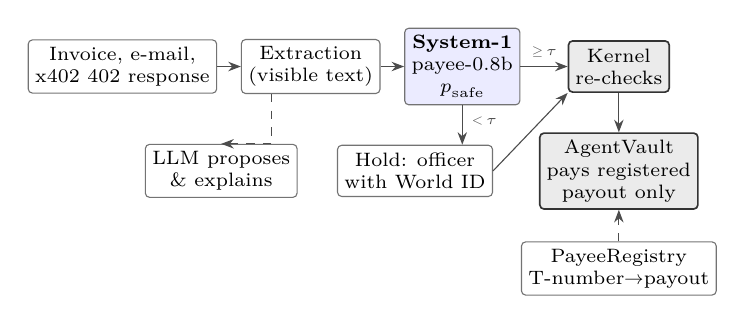
\begin{tikzpicture}[font=\scriptsize, node distance=3.2mm and 3mm,
  box/.style={draw=black!55, rounded corners=1.5pt, align=center, inner sep=2.5pt, minimum height=6.5mm},
  money/.style={box, fill=black!8, draw=black!80, line width=0.6pt},
  arr/.style={-{Stealth[length=1.6mm]}, black!70}]
\node[box] (doc) {Invoice, e-mail,\\x402 402 response};
\node[box, right=of doc] (ext) {Extraction\\(visible text)};
\node[box, right=of ext, fill=blue!8] (s1) {\textbf{System-1}\\payee-0.8b\\$p_\mathrm{safe}$};
\node[box, below=5mm of s1, xshift=-6mm] (hold) {Hold: officer\\with World ID};
\node[money, right=6mm of s1] (kernel) {Kernel\\re-checks};
\node[money, below=5mm of kernel] (vault) {AgentVault\\pays registered\\payout only};
\node[box, left=of hold, xshift=-2mm] (llm) {LLM proposes\\\& explains};
\node[box, below=4mm of vault] (reg) {PayeeRegistry\\T-number$\to$payout};
\draw[arr] (doc) -- (ext);
\draw[arr] (ext) -- (s1);
\draw[arr] (s1) -- node[above, font=\tiny]{$\ge\tau$} (kernel);
\draw[arr] (s1.south) -- node[right, font=\tiny, pos=0.4]{$<\tau$} (hold.north -| s1.south);
\draw[arr] (hold.east) -- (kernel.south west);
\draw[arr] (kernel) -- (vault);
\draw[arr, dashed] (reg) -- (vault);
\draw[arr, dashed] ([xshift=-5mm]ext.south) |- (llm.north);
\end{tikzpicture}
\caption{Where System-1 sits in Meigi. It only routes; the grey boxes are the only components that can move money.}
\label{fig:system}
\end{figure}

\section{PayeeBench-JA}\label{sec:bench}
\textbf{Task.} Each item is the state an agent would assemble: a channel (e-mail, invoice PDF text, chat or x402), the
vendor-master record when one exists (\texttt{payee\_on\_file}: name, T-number, domain, registered destination), and
the document. A model answers four questions: \emph{request type} (routine invoice, payee change, urgent executive
request, credit note, other), \emph{new destination} (does it ask to pay an account or wallet other than the one on
file?), \emph{pressure} (urgency, secrecy or authority used to speed payment or skip checks), and \emph{suspicion} on
a 0--3 scale from clearly benign to very likely redirection fraud.

\textbf{Families and labels.} Table~\ref{tab:families} lists the \NNFamilies{} families. Labels follow from each
item's sampled variant through fixed written rules; for example, a silently swapped 振込先 is a routine invoice with a
new destination, and an overdue notice to the registered account carries pressure but suspicion 1. Hard negatives
include announced bank changes, urgent but legitimate reminders and executives expediting a known invoice; attacks
include keigo requests, executive impersonation, swapped destinations, address-poisoned x402 \texttt{payTo} fields,
and instructions to AI agents hidden in HTML, white text or PDF metadata.

The labels are nearly a function of the family: in \NConstantFamilies{} of the \NNFamilies{} families all four labels
are the same for every item, and answering each test item with its family's most common training labels would score
\NFamilyMajority{}. PayeeBench-JA therefore measures whether a model recognises our families and applies our rules.
\NConventionAnswers{} test answers (starred in Table~\ref{tab:families}) follow a convention that the question text does
not settle, such as suspicion 1 rather than 0 for a properly announced bank change. Some red flags decide the label by
construction: all \NFreeMailAll{} items with a free-mail sender and all \NSwiftAll{} with an overseas (SWIFT) account
are suspicion 3, and no legitimate item has either, so false alarms on legitimate overseas vendors or small businesses
using free mail are not measured.

\begin{table}[t]
\centering
\caption{Families (items in train/val/test) and the labels they take: request type, new destination, pressure,
suspicion. Mixed values are shown with a slash or range; $^*$marks a label that follows one of our conventions.}
\label{tab:families}
\scriptsize
\setlength{\tabcolsep}{3pt}
\begin{tabular}{@{}lrllll@{}}
\toprule
Family & Items & Type & New & Press. & Susp. \\
\midrule
\rows{generated/table_families.tex}
\bottomrule
\end{tabular}
\end{table}

\textbf{Splits and anti-memorization.} There are \NNTrain{}/\NNVal{}/\NNTest{} items (train/validation/test) with the
same family mix. Validation reuses training templates with its own entities; the test split draws layouts, phrasings,
companies, people, banks and x402 merchants from pools that training never sees. Measured: \NTemplatesTestShared{} of
\NTemplatesTest{} test phrase or layout choices and no company, person, bank account, wallet or T-number occur in
training; \NSentTestShared{} of \NSentTest{} test sentences do, all boilerplate; and the mean character 5-gram Jaccard
similarity to the nearest training item is \NJaccardTest{} for test against \NJaccardVal{} for validation. The novelty is
paraphrase within one world model: we wrote both sides for the same slots, with \NInvoiceLayoutsTest{} test invoice
layouts, \NXLayoutsTest{} x402 layout and \NInjectionTextsTest{} injection texts. Every identifier is provably fictional:
T-numbers pass the national check digit~\cite{nta_checkdigit} but use registry office 9999, which no corporation has;
none of our \NNTNumbers{} T-numbers or \NNCompanies{} company names matches the \NNNta{} corporations in the national
index (\NNRenamed{} generic names that did were replaced); phones use exchanges Japan never assigns.

\textbf{Metrics.} Per question we report the accuracy of the top answer (a tie goes to the first option) and
macro-F1. Calibration is the expected calibration error (ECE)~\cite{naeini2015obtaining,guo2017calibration}: top label,
\NBins{} equal-width bins, pooled over the $4\times\NNTest{}$ answers (a stated probability on a bin edge counts in the
upper bin). Routing is selective prediction~\cite{geifman2017selective} on $p_\mathrm{safe}$. An item is \emph{safe} to
auto-clear when it is a routine invoice or credit note, keeps the registered destination and has suspicion at most 1
(\NSafeTest{} test items); the other \NHeldTest{} should be \emph{held}: \NHeldAttacks{} attacks and \NHeldBenign{}
legitimate items that still need a person (\NHeldNotices{} notices, \NHeldChanges{} announced bank changes and
\NHeldExec{} executive requests). Threshold-free, we report the AUROC of $p_\mathrm{safe}$ (safe against held items)
and the most safe items one threshold clears while letting at most $k$ held items through. At a \NBudget{} error budget
(the lowest threshold whose cleared set is at most \NBudget{} held items) we report the share of safe items
auto-cleared, \emph{deployed} (threshold chosen on validation, applied to test) and \emph{oracle} (chosen on test);
with \NNTest{} items this budget tolerates no held item in the cleared set. We also report latency and cost per 1,000
items.

\textbf{Protocol and fairness.} Every model sees the same states and question strings but not our labelling rules: the
fine-tunes learned them from \NNTrain{} examples, the zero-shot models never saw them. Kev models are served through the
same \texttt{/v1/systemone} API, in bf16 with MLX on one laptop. LLMs get one system prompt carrying every question's
instructions and every option's criteria (the strings Kev receives), a short domain preamble and a JSON skeleton, and
must return a probability per option. Llama 3.3 70B Instruct~\cite{meta2024llama33} (the FP8 variant on Cloudflare
Workers AI) was called once per item at temperature 0; \NLlamaParseErrors{} of \NNTest{} replies failed to parse.
\FrontierProtocol{} As a validity check, the kept runs give \NHaikuDistinct{}, \NSonnetDistinct{}, \NOpusDistinct{} and
\NFableDistinct{} distinct answers to the \NNTest{} items (Haiku, Sonnet, Opus, Fable), the discarded one
\NDiscardedDistinct{}. Temperatures and deployed thresholds come from validation; the zero-shot LLMs have no validation
run, so only their oracle auto-clear is reported. Differences are paired over the same answers, with 95\% intervals
from an item-clustered bootstrap~\cite{efron1979bootstrap} (\NResamples{} resamples, an item's four answers kept
together) and from a two-level bootstrap that resamples families, then items within them; $p$-values are exact
two-sided sign tests over items. We call a difference significant when the item-level interval excludes zero and
parity when it contains zero, and say when the family-level interval disagrees.

\section{Method}
Our fine-tunes are supervised: cross-entropy on our labels, not reinforcement learning. payee-0.8b starts from
Kev-0.8B~\cite{palmer2026kev} (\texttt{jaredpalmer/kev-0.8b}): a LoRA adapter~\cite{hu2022lora} (rank \NRank{}, all target
modules) and a pointer head that scores each option's hidden state against the question's, on a frozen
Qwen3.5-0.8B-Base~\cite{qwen2026qwen35base} (revision \texttt{\NBaseRevision}); \NParams{} parameters train. We continue
from the released checkpoint (Hub snapshot \texttt{\NInitSnapshot}, Kev trainer at commit \texttt{\NKevCommit}) for
\NEpochs{} epochs on the \NNTrain{} training items: mean cross-entropy over the four questions, AdamW (weight decay
\NWeightDecay{}), learning rate $\NLr$ on a one-cycle schedule, batch \NBatch{} with \NAccum-step accumulation
(\NTrainSteps{} optimizer steps), gradient-norm clipping at \NClipNorm{} (active on \NClippedSteps{} steps), and Kev's
default augmentation (options reshuffled every epoch; ``none of the above'' replacing the answer or added as a wrong
option, and an irrelevant option added, at \NPNone{}, \NPNoneDistract{} and \NPDistract{}). We then fit one temperature on validation by minimum negative log-likelihood
(T\,=\,\NTempOurs{}). Training took \NTrainMin{} minutes on an Apple M5 Max (48\,GB; fp32 on MPS, each
state encoded once for its four questions), \NTrainStep{}\,s per step at the median and at most \NTrainPeakGpu{}\,GB of
GPU memory. We also fine-tuned Kev-4B (snapshot \texttt{\NInitSnapshotFour}, \NParamsFour{} trainable parameters). The
same recipe did not fit in 48\,GB, so it used a bf16 frozen backbone, gradient checkpointing and one epoch
(\NFourSteps{} steps, \NFourMin{} minutes, T\,=\,\NTempFour{}); it was trained after the 0.8B's test results were known.
\NOpenModels{}

\section{Results}
Table~\ref{tab:results} gives the test results and Fig.~\ref{fig:forest} the paired differences. payee-0.8b reaches
\NOursMean{} mean accuracy: \NVsBaseDelta{} points over the released Kev-0.8B (95\% CI [\NVsBaseLo, \NVsBaseHi];
family-clustered [\NVsBaseFamLo, \NVsBaseFamHi]; better on \NVsBaseBetter{} items and worse on \NVsBaseWorse{}, sign
test $p=\NVsBaseP$), and \NVsBaseFourDelta{} over the five-times-larger released Kev-4B ([\NVsBaseFourLo,
\NVsBaseFourHi]; [\NVsBaseFourFamLo, \NVsBaseFourFamHi]). Most of the gain is on suspicion, where the released models
are near chance on the 0--3 scale (\NBaseSusp{} accuracy, mean error \NBaseSuspMae{} levels) and the fine-tune reaches
\NOursSusp{} (\NOursSuspMae{} levels); the other three questions were already between \NBaseOtherMin{} and
\NBaseOtherMax{} zero-shot. The gain is not mostly our conventions: without the convention answers it is
\NVsBaseNcDelta{} and \NVsBaseFourNcDelta{} points. The fine-tuned 4B is statistically tied with the 0.8B in accuracy
(the 0.8B's lead is \NVsOursFourDelta{} points, CI [\NVsOursFourLo, \NVsOursFourHi], $p=\NVsOursFourP$) but ranks safe
against held items better (AUROC \NOursFourAuroc{} against \NOursAuroc{}; difference CI [\NVsOursFourAurocLo,
\NVsOursFourAurocHi], though the family-clustered interval [\NVsOursFourAurocFamLo, \NVsOursFourAurocFamHi] contains
zero).\NOpenResults{}

Against Llama 3.3 70B the lead is \NVsLlamaDelta{} points ([\NVsLlamaLo, \NVsLlamaHi]; family-clustered
[\NVsLlamaFamLo, \NVsLlamaFamHi]), but it is a lead in following our labels, not in spotting fraud. On the
\NConventionAnswers{} convention answers Llama scores \NLlamaConvAcc{} and payee-0.8b \NOursConvAcc{}; without them the
lead is \NVsLlamaNcDelta{} points ([\NVsLlamaNcLo, \NVsLlamaNcHi]). It sits on request type
(\NVsLlamaRequesttypeDelta{}) and the exact suspicion level (\NVsLlamaSuspicionDelta{}); new destination is tied
(\NVsLlamaNewdestinationDelta{}, [\NVsLlamaNewdestinationLo, \NVsLlamaNewdestinationHi]), and so is the binary split that
$p_\mathrm{safe}$ uses, suspicion 0--1 against 2--3: Llama scores \NLlamaBinSusp{} against \NOursBinSusp{}
(\NVsLlamaBinDelta{} points, [\NVsLlamaBinLo, \NVsLlamaBinHi]) \NLlamaBinPhrase{}.
Llama's clearest miss is invoices that hide an instruction to redirect payment: it flags the new destination on
\NLlamaInjNewDest{} and the suspicion level on \NLlamaInjSusp{} of the \NInjectionN{}, against \NOursInjNewDest{} and
\NOursInjSusp{} for payee-0.8b. The fine-tune is weakest on silently swapped invoices (\NOursSwap{}): \NSwapPoisoned{}
of the \NSwapN{} test items swap in a look-alike wallet that keeps the registered address's first six and last four
hex digits, which only a character-by-character comparison catches. \NFrontierResults{}

\begin{table*}[t]
\centering
\caption{PayeeBench-JA test split (\NNTest{} items): accuracy per question, mean accuracy, ECE, AUROC of
$p_\mathrm{safe}$, safe items auto-cleared at a \NBudget{} error budget (deployed threshold, held items let through, /
oracle), p50 latency and cost per 1,000 items (Section~\ref{sec:cost}). $^\dagger$Test split only; latency includes the
network. $^\ddagger$Run as an agent on the label-free kit; cost estimated from Llama's token counts. --:~not measured.}
\label{tab:results}
\footnotesize
\setlength{\tabcolsep}{4.2pt}
\begin{tabular}{@{}lcccccccccc@{}}
\toprule
Model & Req.\ type & New dest. & Pressure & Suspicion & Mean & ECE & AUROC & Auto-clear @\NBudget{} & p50 (ms) & \$ / 1k \\
\midrule
\rows{generated/table_results.tex}
\bottomrule
\end{tabular}
\end{table*}

\begin{figure}[t]
\centering
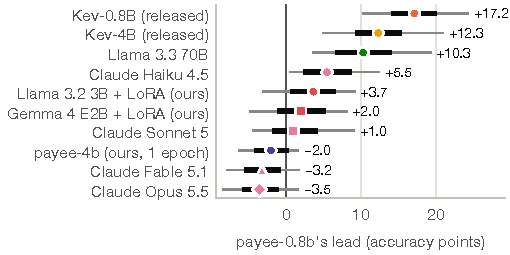
\includegraphics[width=\columnwidth]{figures/forest.pdf}
\caption{payee-0.8b's lead in mean test accuracy over each contender: point estimate, item-bootstrap 95\% interval
(thick) and family-clustered interval (thin). Negative values favour the contender.}
\label{fig:forest}
\end{figure}

\textbf{External check.} We converted AgentDojo's banking suite~\cite{debenedetti2024agentdojo} into PayeeBench items:
its \NExtGoals{} injection goals $\times$ \NExtAttacks{} attack strings $\times$ \NExtCarriers{} carrier documents
(\NExtInjected{} injected items) and \NExtClean{} clean documents, labelled by our rules; and we added the \NExtPfn{}
benign Japanese e-mails of PFN's Japanese-Mail-Bench~\cite{pfn2026mailbench} (Table~\ref{tab:external}; data in
\texttt{results/external}). At its deployed
threshold payee-0.8b auto-clears \NExtOursCleared{} injected items (\NExtOursOffGoal{} of them the password-change goal,
which moves no money), and on the \NExtScope{} in-scope items flags a new destination on \NExtOursNewDest{} and suspicion
2 or more on \NExtOursSusp{}, against \NExtBaseNewDest{} and \NExtBaseSusp{} for the released 0.8B. It flags suspicion 2 or more on
\NExtOursPfnSusp{} benign e-mails (\NExtOursPfnSuspPct{}) and never a new destination. The items are English, Western
and correlated (one attacker IBAN, fixed strings), only one clean document can be cleared, and the labels are our
mapping, not AgentDojo's attack-success metric.

\begin{table}[t]
\centering
\caption{External checks at each model's deployed threshold: injected items auto-cleared (of \NExtInjected{}), and
new-destination and suspicion $\ge$\,2 flags on the \NExtScope{} in-scope items, the \NExtRedirect{} that move money
and \NExtPfn{} benign Japanese e-mails.}
\label{tab:external}
\scriptsize
\setlength{\tabcolsep}{2.4pt}
\begin{tabular}{@{}lcccccc@{}}
\toprule
 & & \multicolumn{2}{c}{In scope} & Money moves & \multicolumn{2}{c}{Benign mail} \\
Model & Cleared & New dest. & Susp. & New / Susp. & New dest. & Susp. \\
\midrule
\rows{generated/table_external.tex}
\bottomrule
\end{tabular}
\end{table}

\section{Calibration and routing}
\begin{figure*}[t]
\centering
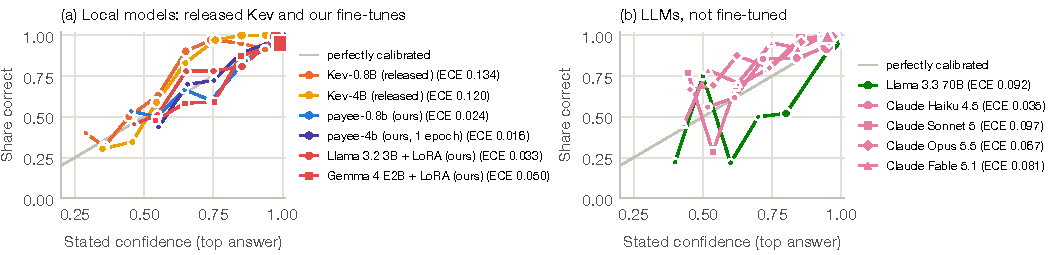
\includegraphics[width=\textwidth]{figures/reliability.pdf}
\caption{Reliability on the test split: share of answers correct against stated confidence, in \NBins{} bins over the
four questions pooled. Marker area grows with the answers in a bin; bins with fewer than \NMinBin{} are omitted.}
\label{fig:reliability}
\end{figure*}
The released Kev models are under-confident (Fig.~\ref{fig:reliability}): Kev-0.8B states \NBaseMeanConf{} mean
confidence at \NBaseMean{} accuracy and Kev-4B \NBaseFourMeanConf{} at \NBaseFourMean{}. Llama is over-confident: its
\NLlamaBinN{} answers stated at about \NLlamaBinConf{} were right \NLlamaBinAcc{} of the time (ECE \NLlamaEce{}).
\NFrontierCalibration{} payee-0.8b's ECE of \NOursEce{} is \NOursEceStanding{}. Pooled ECE hides confident errors,
though: \NOursConfErrors{} of its answers are wrong at \NConfident{} confidence or more (released Kev-4B
\NBaseFourConfErrors{}, Llama \NLlamaConfErrors{}), and it rated \NRemindersRated{} of the \NRemindersN{} benign gentle
reminders in the test split (\NRemindersLang{}) ``very likely a scam'' with probability
\NRemindersPmin{} to \NRemindersPmax{}.

Threshold-free, payee-0.8b ranks safe above held items with an AUROC of \NOursAuroc{},
better than the released Kev-0.8B (\NBaseAuroc{}) but not than the released Kev-4B (\NBaseFourAuroc{}; difference
\NVsBaseFourAurocDelta{}, CI [\NVsBaseFourAurocLo, \NVsBaseFourAurocHi]) or Llama (\NLlamaAuroc{};
\NVsLlamaAurocDelta{}, [\NVsLlamaAurocLo, \NVsLlamaAurocHi], though the family-clustered interval [\NVsLlamaAurocFamLo,
\NVsLlamaAurocFamHi] contains zero). With no held item cleared, or one, where a \NBudget{} budget operates, it clears
\NOursClearZero{} and \NOursClearOne{} of the \NSafeTest{} safe items, against \NBaseFourClearZero{} and
\NBaseFourClearOne{} for Kev-4B and \NLlamaClearZero{} and \NLlamaClearOne{} for Llama; these are differences of
\NClearGapMin{} to \NClearGapMax{} items whose intervals contain zero (against Llama, [\NVsLlamaClearZeroLo, \NVsLlamaClearZeroHi] and
[\NVsLlamaClearOneLo, \NVsLlamaClearOneHi] points of the safe items). \NFrontierRouting{}

With the threshold fixed on validation ($\tau$\,=\,\NOursThreshold), payee-0.8b clears \NOursDeployed{} of the safe test
items (\NOursDeployedN{} of \NSafeTest{}; \NOursDeployedLo{} to \NOursDeployedHi{} when test items are resampled) and
lets \NOursFalseClears{} held item through: an invoice whose 振込先 moved to another bank under the same account name,
which the kernel's registry match exists to catch. The fine-tuned 4B clears \NOursFourDeployed{}, also with
\NOursFourFalseClears{} held item; the released Kev-4B \NBaseFourDeployed{}, and the released 0.8B nothing, even with a
refitted temperature. This is not like-for-like: validation shares training templates and fitted the temperature, so
the fine-tunes rank it almost perfectly (AUROC \NOursAurocVal{} for payee-0.8b) and their threshold is loose on test,
while the released Kev-4B ranks validation worse than test (\NBaseFourAurocVal{} against \NBaseFourAuroc{}). A
production threshold should come from real held-out documents, with a margin.


\section{Cost and speed}\label{sec:cost}
Latency is the client's wall time for one HTTP request answering all four questions, one request at a time, after
warm-up. payee-0.8b answers in \NOursPfifty{}\,ms at p50 (\NOursPninetyfive{}\,ms at p95), the same as the released
0.8B; the 4B models take about \NOursFourPfifty{}\,ms. These are over localhost; Llama's \NLlamaPfifty{}\,ms
(\NLlamaPninetyfive{}\,ms at p95) includes the network and our proxy. A local model has no token bill, so we price the
time a request occupies the machine, $t_\text{item}\cdot W\cdot c_\mathrm{kWh}$, with $t_\text{item}$ the mean wall
time per item, $W$\,=\,\NWatts{}\,W an assumed package power and $c_\mathrm{kWh}$\,=\,\$\NUsdKwh{} per kWh (a Tokyo
household tariff), excluding the hardware: \$\NOursCost{} per 1,000 items for payee-0.8b. Hosted models are priced
at list price for their measured tokens: Llama 3.3 70B costs \$\NLlamaCost{} per 1,000 items~\cite{cloudflare_pricing}.
\NFrontierCost{} Llama costs about \NLlamaOverOurs{} times our electricity, but electricity on owned hardware against a
list price is not a like-for-like ratio. On a rented NVIDIA L4
at \$\NLfourHour{} per hour and Kev's published throughput of \NLfourRps{} requests per second (a different workload:
short texts, many concurrent clients), Kev-0.8B would cost about \$\NLfourCost{} per 1,000 items, still about
\NLlamaOverLfour{} times less than Llama.


\section{Forgetting}
On Kev's own out-of-domain development suite
(transfer-v4, \NFgN{} answers, served the same way) accuracy held: \NFgBaseAcc{} to \NFgOursAcc{} for the 0.8B and
\NFgBaseFourAcc{} to \NFgOursFourAcc{} for the 4B. Calibration did not: ECE rose from \NFgBaseEce{} to \NFgOursEce{}
(0.8B) and from \NFgBaseFourEce{} to \NFgOursFourEce{} (4B), and wrong answers given with at least 0.9 confidence rose
from \NFgBaseConf{} to \NFgOursConf{} (0.8B). The fitted temperature belongs to the payee questions; Meigi serves the
fine-tune for this question set only.

\section{Limitations}
PayeeBench-JA is synthetic and self-built: it measures how well a model learns our families and conventions, not fraud
detection in real mail with OCR noise, threads and attachments. The test set is small and clustered: intervals are
several points wide, family-clustered ones about twice as wide, and one or two items decide the \NBudget{} auto-clear
figure. The test split was reused: the models were trained on an earlier build that differs only in identifiers,
every model was scored once per build, the 4B was trained after the 0.8B's results were known, and the 0.8B was chosen
on test. Each model was trained once, with one seed. The frontier rows are agents with context, reasoning and a shell,
run once, with no latency and an estimated cost. TypeSafe's hosted System-1 model, Jev~\cite{typesafe_models}, was not
evaluated.

\textbf{Audit.} An AI auditing agent re-derived the headline numbers with independent code and found one bug, fixed
throughout: a probability exactly on a bin edge fell into the lower bin, understating Llama's ECE
(\NLlamaEceBeforeFix{}, now \NLlamaEce{}). Its other findings narrowed our claims and made the agent rows indicative. A
second AI review recomputed the headline numbers, frontier rows included; the open-model rows came after it.

\section{Conclusion}
On PayeeBench-JA, a 0.8B decision model fine-tuned on \NNTrain{} synthetic items in \NTrainMin{} minutes on a laptop
learns our labels: it is \NVsBaseDelta{} points more accurate than the released model, its calibration error is
\NOursEceStanding{}, and it answers in \NOursPfifty{}\,ms at a negligible marginal cost. It is not a better detector of
redirection than large LLMs, which rank safe against held items at least as well\NOpenConclusion{}.\NFrontierConclusion{} What it offers
a payment agent is a local, cheap first pass with mostly calibrated probabilities that never needs to be trusted with
money: the model only routes, and money moves only through exact, on-chain checks.

\section*{Reproducibility}
Everything is under \texttt{bench/} in the Meigi repository: the dataset builder (byte-identical output given the
national corporation index, which is not in the repository), the fine-tuning and evaluation scripts, the label-free kit
and its scorer, the agents' instructions, and the \texttt{paper/} scripts that generate every number, table and figure
from \texttt{results/} and \texttt{dataset/}. The fine-tuned weights are not published: their predictions can be
re-scored, not re-run.

\section*{Acknowledgment}
This paper was written with AI assistance (Claude) and audited by AI agents. All numbers come from
\texttt{bench/results} and \texttt{bench/dataset}, through the scripts above.

\bibliographystyle{IEEEtran}
\bibliography{refs}

\end{document}
